% Options for packages loaded elsewhere
\PassOptionsToPackage{unicode}{hyperref}
\PassOptionsToPackage{hyphens}{url}
%
\documentclass[
]{article}
\usepackage{amsmath,amssymb}
\usepackage{iftex}
\ifPDFTeX
  \usepackage[T1]{fontenc}
  \usepackage[utf8]{inputenc}
  \usepackage{textcomp} % provide euro and other symbols
\else % if luatex or xetex
  \usepackage{unicode-math} % this also loads fontspec
  \defaultfontfeatures{Scale=MatchLowercase}
  \defaultfontfeatures[\rmfamily]{Ligatures=TeX,Scale=1}
\fi
\usepackage{lmodern}
\ifPDFTeX\else
  % xetex/luatex font selection
\fi
% Use upquote if available, for straight quotes in verbatim environments
\IfFileExists{upquote.sty}{\usepackage{upquote}}{}
\IfFileExists{microtype.sty}{% use microtype if available
  \usepackage[]{microtype}
  \UseMicrotypeSet[protrusion]{basicmath} % disable protrusion for tt fonts
}{}
\makeatletter
\@ifundefined{KOMAClassName}{% if non-KOMA class
  \IfFileExists{parskip.sty}{%
    \usepackage{parskip}
  }{% else
    \setlength{\parindent}{0pt}
    \setlength{\parskip}{6pt plus 2pt minus 1pt}}
}{% if KOMA class
  \KOMAoptions{parskip=half}}
\makeatother
\usepackage{xcolor}
\usepackage[vmargin=1in,hmargin=1in]{geometry}
\usepackage{longtable,booktabs,array}
\usepackage{calc} % for calculating minipage widths
% Correct order of tables after \paragraph or \subparagraph
\usepackage{etoolbox}
\makeatletter
\patchcmd\longtable{\par}{\if@noskipsec\mbox{}\fi\par}{}{}
\makeatother
% Allow footnotes in longtable head/foot
\IfFileExists{footnotehyper.sty}{\usepackage{footnotehyper}}{\usepackage{footnote}}
\makesavenoteenv{longtable}
\usepackage{graphicx}
\makeatletter
\def\maxwidth{\ifdim\Gin@nat@width>\linewidth\linewidth\else\Gin@nat@width\fi}
\def\maxheight{\ifdim\Gin@nat@height>\textheight\textheight\else\Gin@nat@height\fi}
\makeatother
% Scale images if necessary, so that they will not overflow the page
% margins by default, and it is still possible to overwrite the defaults
% using explicit options in \includegraphics[width, height, ...]{}
\setkeys{Gin}{width=\maxwidth,height=\maxheight,keepaspectratio}
% Set default figure placement to htbp
\makeatletter
\def\fps@figure{htbp}
\makeatother
\setlength{\emergencystretch}{3em} % prevent overfull lines
\providecommand{\tightlist}{%
  \setlength{\itemsep}{0pt}\setlength{\parskip}{0pt}}
\setcounter{secnumdepth}{-\maxdimen} % remove section numbering
\newlength{\cslhangindent}
\setlength{\cslhangindent}{1.5em}
\newlength{\csllabelwidth}
\setlength{\csllabelwidth}{3em}
\newlength{\cslentryspacingunit} % times entry-spacing
\setlength{\cslentryspacingunit}{\parskip}
\newenvironment{CSLReferences}[2] % #1 hanging-ident, #2 entry spacing
 {% don't indent paragraphs
  \setlength{\parindent}{0pt}
  % turn on hanging indent if param 1 is 1
  \ifodd #1
  \let\oldpar\par
  \def\par{\hangindent=\cslhangindent\oldpar}
  \fi
  % set entry spacing
  \setlength{\parskip}{#2\cslentryspacingunit}
 }%
 {}
\usepackage{calc}
\newcommand{\CSLBlock}[1]{#1\hfill\break}
\newcommand{\CSLLeftMargin}[1]{\parbox[t]{\csllabelwidth}{#1}}
\newcommand{\CSLRightInline}[1]{\parbox[t]{\linewidth - \csllabelwidth}{#1}\break}
\newcommand{\CSLIndent}[1]{\hspace{\cslhangindent}#1}
\usepackage{pdflscape,booktabs}
\newcommand{\blandscape}{\begin{landscape}}
\newcommand{\elandscape}{\end{landscape}}
\usepackage[running]{lineno}
\linenumbers
\ifLuaTeX
  \usepackage{selnolig}  % disable illegal ligatures
\fi
\IfFileExists{bookmark.sty}{\usepackage{bookmark}}{\usepackage{hyperref}}
\IfFileExists{xurl.sty}{\usepackage{xurl}}{} % add URL line breaks if available
\urlstyle{same}
\hypersetup{
  hidelinks,
  pdfcreator={LaTeX via pandoc}}

\author{}
\date{\vspace{-2.5em}}

\begin{document}

\hypertarget{the-response-of-trophic-interaction-networks-to-multiple-stressors-in-a-marine-latitudinal-gradient-of-the-southern-hemisphere}{%
\section{The response of trophic interaction networks to multiple
stressors in a marine latitudinal gradient of the Southern
Hemisphere}\label{the-response-of-trophic-interaction-networks-to-multiple-stressors-in-a-marine-latitudinal-gradient-of-the-southern-hemisphere}}

\hypertarget{running-title-marine-stressors-in-the-southern-hemisphere}{%
\subsection{Running Title: Marine stressors in the Southern
Hemisphere}\label{running-title-marine-stressors-in-the-southern-hemisphere}}

\subsection{Running Title: Marine stressors in the Southern
Hemisphere}\label{running-title-marine-stressors-in-the-southern-hemisphere}

Tomás I. Marina\textsuperscript{1}, Leonardo A.
Saravia\textsuperscript{1,2,*}, Iara D. Rodriguez\textsuperscript{3},
Manuela Funes\textsuperscript{4}, Georgina Cordone\textsuperscript{5},
Santiago R. Doyle\textsuperscript{3,6}, Anahí
Silvestro\textsuperscript{6}, David E. Galván\textsuperscript{5},
Susanne Kortsch\textsuperscript{7} \& Fernando Momo\textsuperscript{3,6}

\textsuperscript{1} Centro Austral de Investigaciones Científicas
(CADIC-CONICET), Ushuaia, Argentina;

\textsuperscript{2} Instituto de Ciencias Polares, Ambiente y Recursos
Naturales, Universidad Nacional de Tierra del Fuego (UNTdF), Ushuaia,
Argentina;

\textsuperscript{3} Instituto de Ciencias, Universidad Nacional de
General Sarmiento (UNGS), Los Polvorines, Argentina;

\textsuperscript{4} Instituto de Investigaciones Marinas y Costeras
(IIMyC-CONICET), Mar del Plata, Argentina;

\textsuperscript{5} Centro Para el Estudio de Sistemas Marinos
(CESIMAR-CONICET), Puerto Madryn, Argentina;

\textsuperscript{6} Instituto de Ecología y Desarrollo Sustentable
(INEDES-CONICET-UNLu), Luján, Argentina;

\textsuperscript{7} Tvärminne Zoological Station, University of
Helsinki, Hanko, Finland.

* corresponding author: Leonardo A. Saravia. Centro Austral de
Investigaciones Científicas (CADIC-CONICET), Ushuaia, Argentina.
\href{mailto:lasaravia@untdf.edu.ar}{\nolinkurl{lasaravia@untdf.edu.ar}}

\hypertarget{abstract}{%
\subsection{Abstract}\label{abstract}}

Ecological networks offer valuable insights into community structure,
key species identification, and ecosystem management for biodiversity
conservation. Understanding how these networks react to environmental
and anthropogenic stressors, especially along geographical gradients, is
of increasing interest. This review presents a pioneering analysis of
stressor responses in marine food webs from the southwest Atlantic to
the Antarctic (45 - 78ºS), encompassing areas such as San Jorge Gulf,
Beagle Channel, Burdwood Bank, Scotia Sea, Potter Cove, and the Weddell
Sea in Antarctica. Our objectives are to: 1) describe the structure of
marine food webs along this axis using a network approach; 2) identify
predominant environmental and anthropogenic stressors affecting each
ecosystem; and 3) summarize observed food web changes and hypothesize on
stressor impacts. Our collaborative team, comprising regional experts
and global authorities on high-latitude marine food webs and stressor
effects, ensures a comprehensive and credible literature review. We
assessed the effects of stressors primarily at the species level, with
notable exceptions like fisheries in San Jorge Gulf. Hypotheses for each
study area were formulated considering: a) stressors; b) impacted
parameters; c) node-level species properties; and d) network-level food
web properties. Global warming emerges as the most common stressor
across the gradient, except in the Beagle Channel and Burdwood Bank,
where alien species introduction and fisheries are more influential,
respectively. We offer specific hypotheses on how warming may affect
food webs. Our findings highlight the benefits of a network approach in
understanding and predicting stressor effects in Southern Hemisphere
marine ecosystems. This approach provides a holistic understanding of
ecological networks, enhances our ability to identify key species and
interactions, and offers insights for ecosystem management and
conservation in the face of various stressors.

Keywords: anthropogenic stressors, environmental stressors, food webs,
latitudinal gradient, Southern Hemisphere

\hypertarget{introduction}{%
\subsection{1. Introduction}\label{introduction}}

The application of a network perspective has emerged as a powerful tool
to tackle the complexity of species interactions, facilitating a better
understanding of the structure and functioning of ecosystems (Belgrano,
Scharler, Scharler, Dunne, \& Ulanowicz, 2005; Thompson et al., 2012).
Trophic networks (or food webs) allow identifying properties and key
species that may be crucial for ecosystem stability, and hence important
for ecosystem management and biodiversity conservation (Thompson et al.,
2012). There is a growing interest in understanding how ecological
networks respond to environmental and anthropogenic stressors along
geographical gradients (Cirtwill, Stouffer, \& Romanuk, 2015; Bauer et
al., 2022). Yet, only a few studies have described variation in food web
structure along latitudinal gradients in marine ecosystems. The few that
have come from the Global North (Wood, Russell, Hanson, Williams, \&
Dunne, 2015; Kortsch et al., 2019; Pecuchet et al., 2022), whereas no
studies, nor meta-analyses, on geographical variation in marine food
webs exist for the Global South (Southern Hemisphere).

Here we review for the first time the state-of-the-art knowledge on
stressor response of marine food webs along the southwest Atlantic to
Antarctic gradient (45 - 78ºS, Figure 1). We focus on proven and
expected changes in food webs driven by stressors in selected areas
along this large-scale latitudinal gradient. We recruited food web
experts from different marine systems of Argentina and the world (see
co-authors' list). Throughout the year 2023 we maintained regular
discussion meetings, typically held every two or three weeks. The aim of
this review is threefold: 1) describe the complexity and structure of
marine food webs along the southwest Atlantic to Antarctic axis from a
network perspective; 2) identify the ongoing environmental and
anthropogenic stressors for each marine ecosystem containing the food
webs; and 3) resume proven food web changes and elaborate hypotheses on
how the identified stressors might affect food web features (e.g.~energy
flow, stability), combining information on node- and network-level
properties. Finally, we suggest which additional data and analyses are
needed to gain insights into the stressors' effects on food web
properties in the southwest Atlantic to Antarctic region.

\hypertarget{the-structure-of-marine-food-webs-in-the-southwest-atlantic---antarctic-region}{%
\subsection{2. The structure of marine food webs in the Southwest
Atlantic - Antarctic
region}\label{the-structure-of-marine-food-webs-in-the-southwest-atlantic---antarctic-region}}

Together, the southwest and the Atlantic sector of the Southern Ocean
comprise one of the most biologically productive regions of the world's
oceans (Acha, Mianzan, Guerrero, Favero, \& Bava, 2004; Latorre et al.,
2023). The referred region extends from San Jorge Gulf (45ºS) in the
Patagonian shelf to the Weddell Sea (78ºS) in the Southern Ocean, and
covers a well-connected oceanic latitudinal gradient (R. P. Matano,
Palma, \& Piola, 2010; Guihou, Piola, Palma, \& Chidichimo, 2020).

Throughout this latitudinal gradient, many investigations have been
carried out addressing the trophic ecology of specific species and
prey-predator relationships (Vinuesa \& Varisco, 2007; Pasotti et al.,
2015; Saunders, Hill, Tarling, \& Murphy, 2019; Riccialdelli et al.,
2020), but few studies have considered the complexity of the ecosystem
in terms of a high resolution of species and their prey-predator
interactions (but see Jacob et al. (2011), Marina et al. (2018), Funes,
Saravia, Cordone, Iribarne, \& Galván (2022), López-López, Genner,
Tarling, Saunders, \& O'Gorman (2022), Rodriguez, Marina, Schloss, \&
Saravia (2022), Marina et al. (in rev.)). Neglecting this complexity
might lead to a misunderstanding of the structure and functioning of the
ecosystems, and ultimately reduce the ability to predict ecosystem
responses to perturbations (Montoya, Woodward, Emmerson, \& Solé, 2009).

In this review, we consider marine areas in the Southern hemisphere for
which highly-resolved empirical food webs, in terms of species diversity
and trophic interactions, have been previously described. These areas
include: (1) San Jorge Gulf (45 - 47ºS, 65 - 68ºW), (2) Beagle Channel
(\textasciitilde54ºS, 68ºW), (3) Burdwood Bank (\textasciitilde54ºS,
59ºW), (4) Scotia Sea (48 - 58ºS, 50ºW), (5) Potter Cove (62ºS, 58ºW,
Antarctica), and (6) Weddell Sea (74 - 78ºS, 30ºW, Antarctica) (Figure
1). The geographic locations of these marine biomes span from temperate
to Antarctic, and are exposed to both environmental (sea warming,
glacial retreat) and anthropogenic (fishery, pollution) stressors.

\begin{figure}
\centering
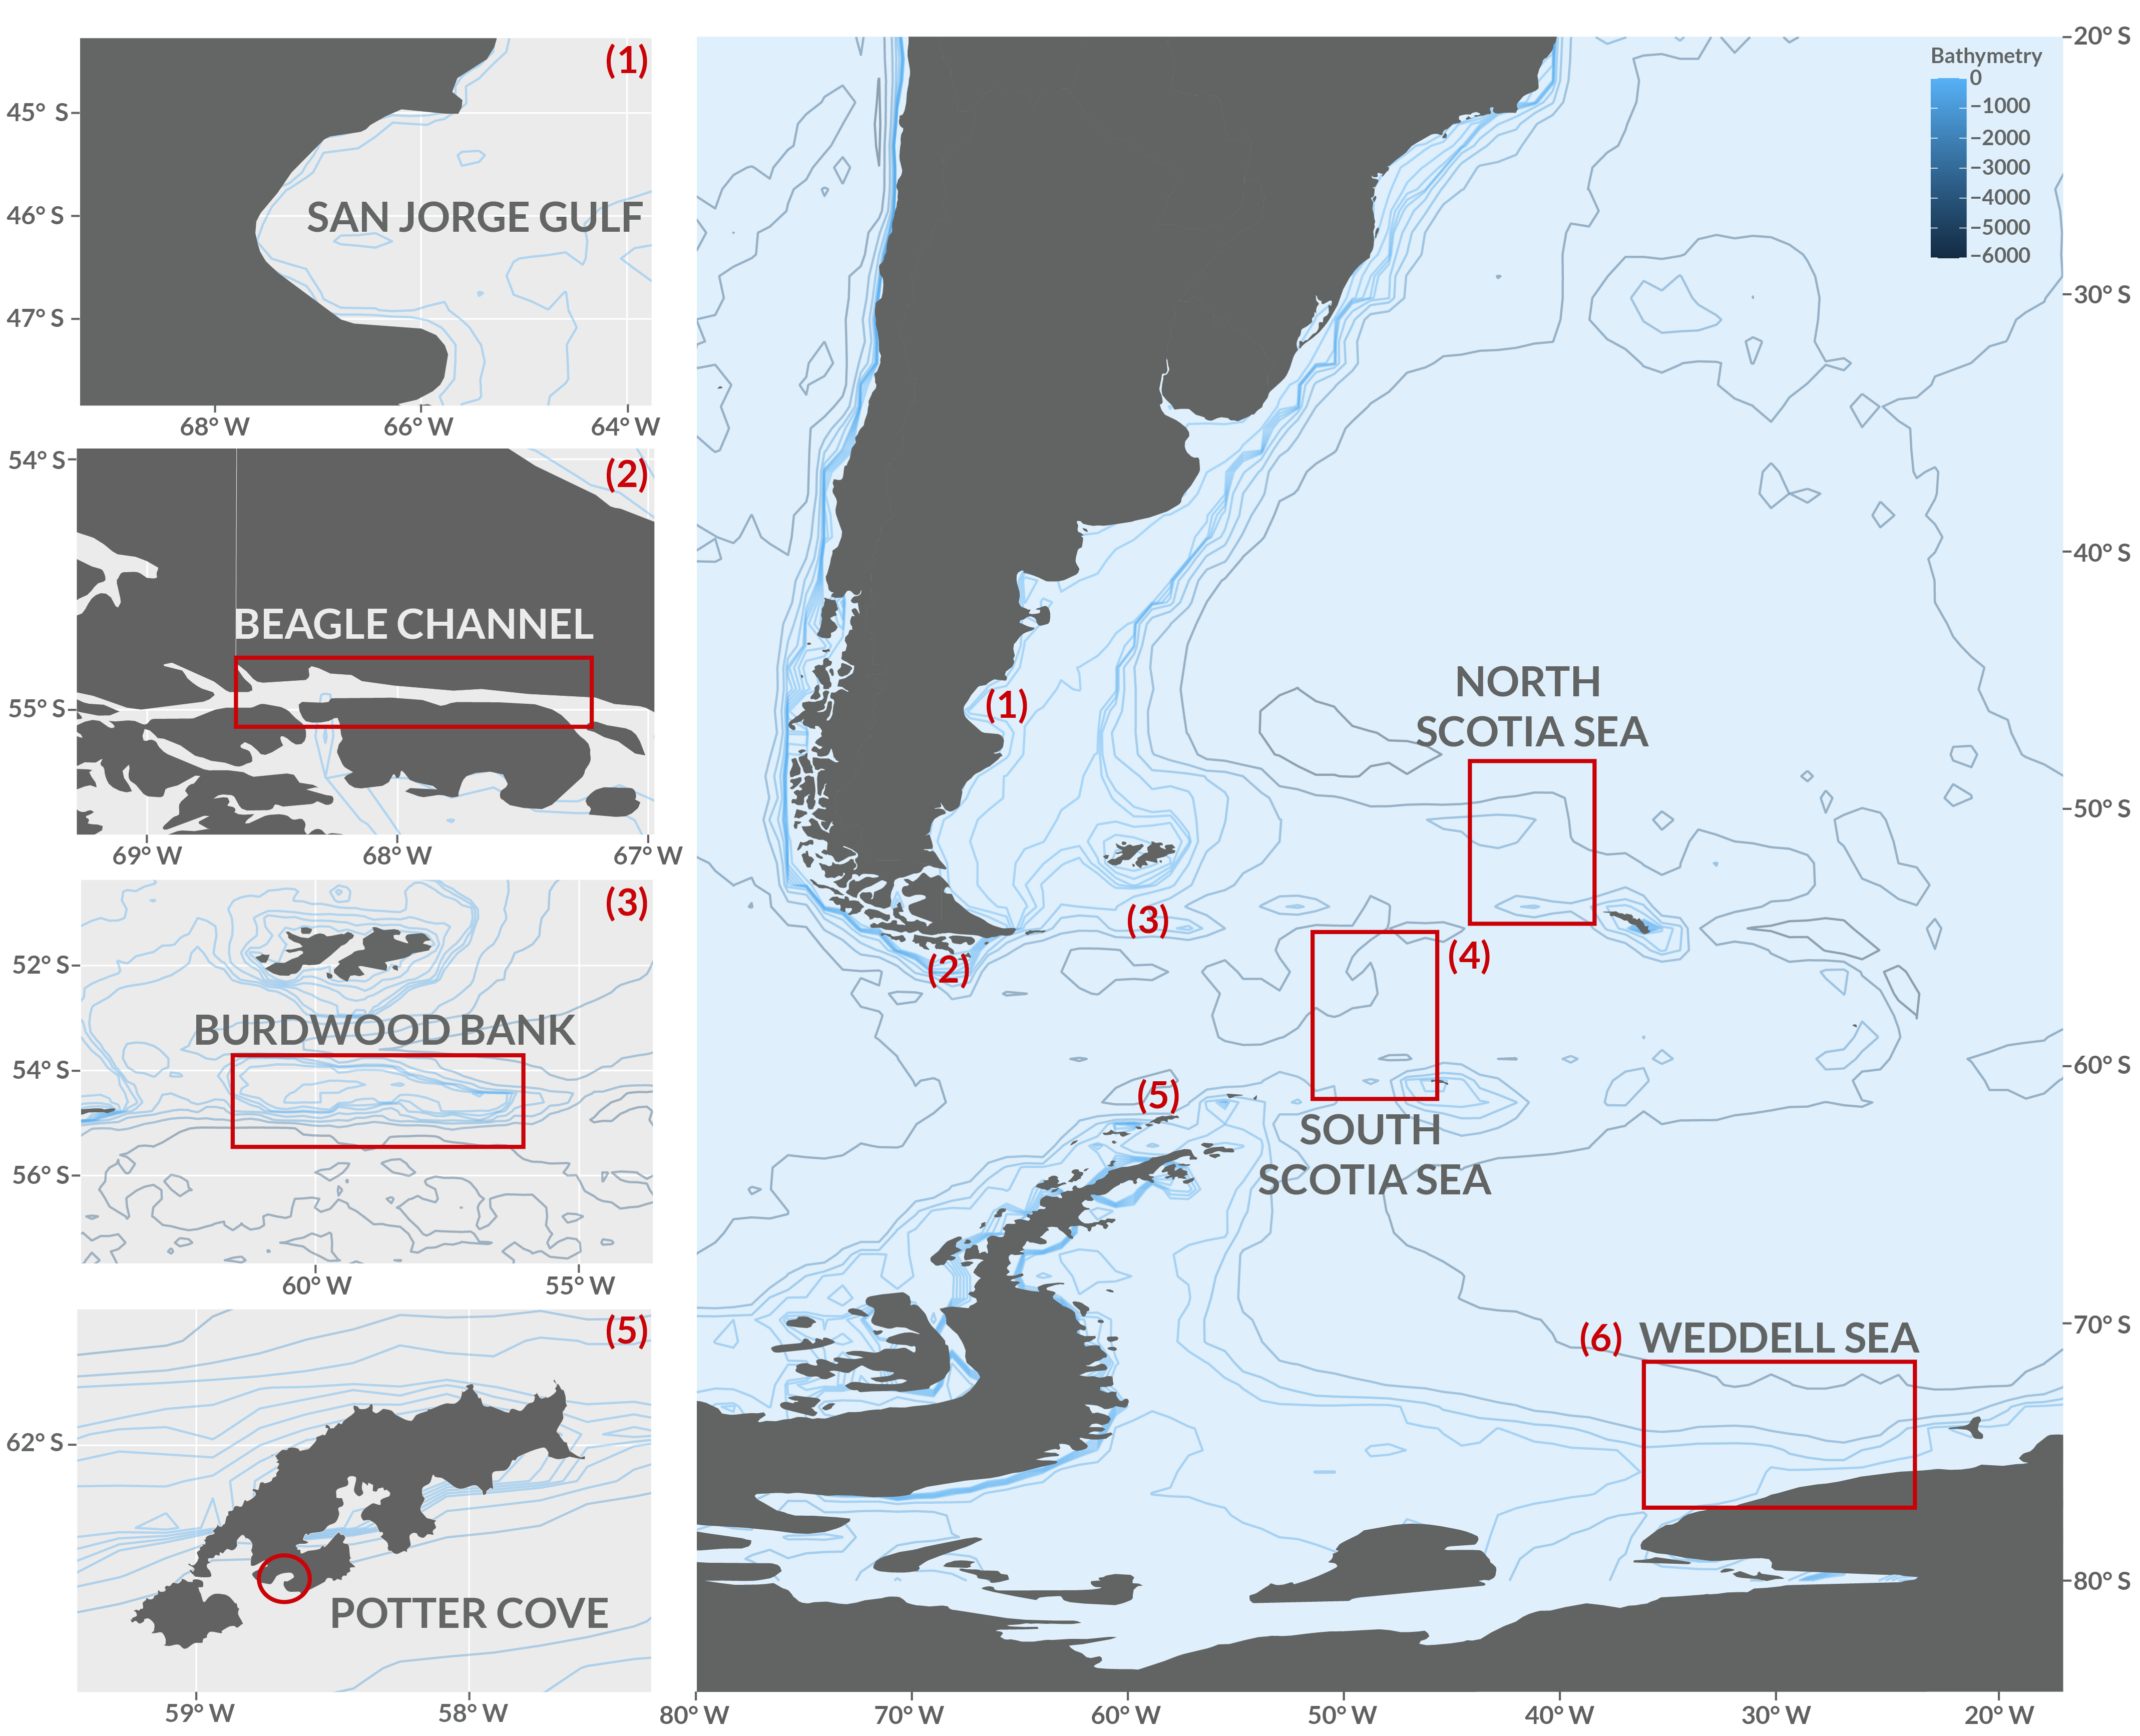
\includegraphics[width=6.27in,height=3.528in]{Figures/Map_final.jpg}
\caption{Map of the study areas along the southwest Atlantic - Antarctic
latitudinal gradient. The areas are marked with numbers from one to six.
Smaller areas (1. San Jorge Gulf, 2. Beagle Channel, 3. Burdwood Bank,
and 5. Potter Cove) are shown on the panels to the left, whereas the
larger areas (4. North and South Scotia Sea, and 6. Weddell Sea) are
marked with a red rectangle on the map. The map was drawn using the
`marmap' R package (Pante, Simon-Bouhet, \& Irisson, 2023). Continental
contour shapefiles were obtained from www.ign.gob.ar.}
\end{figure}

San Jorge Gulf is the northernmost study area considered in this review.
It is a partially enclosed basin spanning approximately 34,000 km2 and
\textasciitilde100 m of maximum depths, located from Cabo dos Bahias
(44°55'S) to Cabo tres Puntas (47°06'S) (Figure 1). The shallower
northern and southern ends of the Gulf (with depths \textasciitilde40 m)
present two prominent frontal systems. These systems are the areas of
highest productivity (Glembocki, Williams, Góngora, Gagliardini, \&
Orensanz, 2015). The Gulf's productivity supports large invertebrate and
vertebrate fisheries (Góngora, González-Zevallos, Pettovello, \& Mendía,
2012), as well as marine mammal and seabird populations (Yorio, 2009).
The San Jorge Gulf food web comprises 165 nodes and 1015 trophic
interactions with a connectance of 0.04. The percentage of top predators
is 16\%, 78\% of intermediate nodes and 6\% of basal nodes; 60\% of
predators are omnivorous (Table 1). The most connected nodes are: the
Argentine red shrimp Pleoticus muelleri, the squat lobster Gimothea
gregaria, squids (Illex argentinus as dominant species) and Amphipoda.
Notably, these nodes present mid-trophic positions in the food web (3.0,
2.5, 3.6 and 2, respectively) (Funes et al., 2022).

At a southern latitude, the Beagle Channel (54°52'S, 68°8'W) is an
interoceanic passage located at the southernmost tip of South America,
spanning 240 km in length and 5 km in width (\textasciitilde1200 km2),
and a range depth of 0 - 140 m (Figure 1). It features complex
coastlines, varying bathymetry, a prevailing west-to-east circulation
pattern, and a significant longitudinal gradient of glacial freshwater
discharge (Schloss et al., 2023). Bruno, Riccialdelli, Acha, \&
Fernández (2023) suggests that locally produced suspended particulate
organic matter (mostly composed by phytoplankton) and organic matter
accumulated in the sediments (macroalgae-originated detritus) are the
primary food sources for the marine ecosystem, as opposed to
allochthonous materials. Beagle Channel food web includes 145 nodes and
1115 trophic interactions with a connectance of 0.05 (Table 1). The food
web is suggested to have a wasp-waist structure, where the following
species play a crucial role in the dynamics of the ecosystem: Fueguian
sprat Sprattus fuegensis, longtail southern cod Patagonotothen ramsayi,
black southern cod P. tessellata, frogmouth Cottoperca trigloides, and
squat lobster Grimothea gregaria (Riccialdelli et al., 2020). Moreover,
the squat lobster has been identified as a species responsible for
linking modules and connecting the entire food web (Rodriguez et al.,
2022).

The so-called Burdwood Bank ecosystem comprises Marine Protected Areas
Namuncurá - Burdwood Bank I and II, meaning the shallow submarine
plateau named Burdwood Bank with a 200 m isobath boundary, and a deep
slope that reaches 4000 m in depth, respectively (Administración de
Parques Nacionales, 2022) (Figure 1). Physical features in the plateau
are fairly stable, with salinity averaging 34 all year round and
temperature ranging between 4 and 8ºC (Acha et al., 2004). The plateau
is surrounded by steep flanks of up to 4000 m depth, protected by the
Marine Protected Area Namuncurá - Burdwood Bank II (32,000 km2;
\textasciitilde55º - 56ºS, \textasciitilde58º - 62ºW). Intense upwelling
and mixing occur in relation to the slope, entraining deep nutrient-rich
waters into the photic layer (Ricardo P. Matano, Palma, \& Combes,
2019), and resulting in a fairly homogeneous water column both spatially
and temporally (Ricardo P. Matano et al., 2019). The Burdwood Bank food
web comprises 379 nodes and 1788 interactions, with a connectance of
0.01, and an asymmetric degree distribution (i.e.~most of the species
have a relatively low number of interactions and few species concentrate
most of them). Almost half of the consumers are omnivores (0.48), and
the network displays a small-world pattern (Marina et al., in rev.)
(Table 1).

The Scotia Sea is a deep-sea basin, delimited by the Drake Passage to
the West and by the island complex of the Scotia Arc to the North, East,
and South, with an approximate extension of 1.5 x 106 km2 and a depth
range of 0 - 3000 m (E. j. Murphy et al., 2006) (Figure 1). Its
oceanography is dominated by the Antarctic Circumpolar Current, which is
spatially structured by frontal systems (Whitworth, 1980). The South
Antarctic Circumpolar Current Front subdivides the Scotia Sea into two
biogeographic regions: the Northern Scotia Sea is characterized by
higher and more variable temperatures, and the Southern Scotia Sea by
lower and more stable temperatures and influenced by seasonal sea ice
(Raymond, 2011). The analysis of the Northern and Southern Scotia Sea
food webs shows that the former is relatively more complex than the
latter: with higher species richness (218 vs 192) and interactions
(10008 vs 7241) and a higher connection overall (0.21 vs 0.20). As
expected from a more complex network, the path length is shorter in the
Northern Scotia Sea food web. In the same sense, the Southern Scotia Sea
network displays a greater proportion of omnivores and a lower mean
trophic level (López-López et al., 2022) (Table 1).

In the Antarctic realm, Potter Cove is a \textasciitilde9 km2 fjord with
a depth range of 0 - 200 m located at 25 de Mayo/King George Island
(62°14'S, 58°38'W, South Shetland Islands) on the West Antarctic
Peninsula (Figure 1). The cove, bordered by the Fourcade Glacier, is
divided into three areas: a) the internal cove, a high
glacier-influenced, soft sediment zone with a 50 m maximum depth; b) the
central cove, a mixed substrate area with low meltwater influence and an
80 m maximum depth; and c) the external cove, ice-free for 60 years with
a 185 m maximum depth and rocky substrate (Jerosch et al., 2018). Potter
Cove's high-latitude location results in variable environmental
conditions due to photoperiod length seasonality. Sea ice often covers
this area in winter (Schloss et al., 2012). With low phytoplankton
biomass, macroalgae, and microphytobenthos are likely the primary food
sources for secondary benthic production (M. L. Quartino \& Boraso de
Zaixso, 2008). The Potter Cove food web includes 110 nodes and 649
interactions, with an asymmetric degree distribution, and a connectance
value of 0.05 (Table 1). It presents a modular structure (groups of
species interact more strongly with each other than with species
belonging to other groups), that's positively associated with stability,
since perturbation can be retained within modules (Rodriguez et al.,
2022).

Located between 74 and 78ºS, the high Antarctic Weddell Sea shelf spans
approximately 450 km from East to West (Jacob et al., 2011) (Figure 1).
The water depth ranges from 200 to 500 m, with shallower regions being
covered by continental ice that forms the coastline along the eastern
and southern parts of the Weddell Sea. Within this shelf area, exists a
complex three-dimensional benthic habitat characterized by substantial
benthic biomasses and an intermediate to high diversity when compared to
benthic boreal communities (Teixidó, Garrabou, \& Arntz, 2002). The
Weddell Sea food web exhibits a high level of network complexity,
featuring the greatest number of nodes (490) and trophic interactions
(16041) among the analyzed food webs in this review (Table 1). Its
connectance (0.07) and other structural properties are intermediate
compared to the other food webs. Recently, the interaction strengths of
this food web were estimated, revealing the presence of numerous weak
and few strong interactions, which is consistent with findings in other
complex food webs (Nilsson \& McCann, 2016). Notably, this asymmetric
distribution of interaction strength is likely to promote community
persistence.

\newpage
\footnotesize

Table 1. Complexity and structure properties of the marine food webs
considered in the present review. Refer to Table 2 for definition of
properties. mean TL: mean trophic level. Food webs are ordered by
increasing latitude.

\begin{longtable}[]{@{}
  >{\raggedright\arraybackslash}p{(\columnwidth - 14\tabcolsep) * \real{0.1538}}
  >{\centering\arraybackslash}p{(\columnwidth - 14\tabcolsep) * \real{0.0839}}
  >{\centering\arraybackslash}p{(\columnwidth - 14\tabcolsep) * \real{0.0839}}
  >{\centering\arraybackslash}p{(\columnwidth - 14\tabcolsep) * \real{0.1259}}
  >{\centering\arraybackslash}p{(\columnwidth - 14\tabcolsep) * \real{0.1259}}
  >{\centering\arraybackslash}p{(\columnwidth - 14\tabcolsep) * \real{0.0979}}
  >{\centering\arraybackslash}p{(\columnwidth - 14\tabcolsep) * \real{0.1049}}
  >{\centering\arraybackslash}p{(\columnwidth - 14\tabcolsep) * \real{0.2238}}@{}}
\toprule\noalign{}
\begin{minipage}[b]{\linewidth}\raggedright
\textbf{Food web}
\end{minipage} & \begin{minipage}[b]{\linewidth}\centering
\textbf{Nodes}
\end{minipage} & \begin{minipage}[b]{\linewidth}\centering
\textbf{Links}
\end{minipage} & \begin{minipage}[b]{\linewidth}\centering
\textbf{Connectance}
\end{minipage} & \begin{minipage}[b]{\linewidth}\centering
\textbf{Path length}
\end{minipage} & \begin{minipage}[b]{\linewidth}\centering
\textbf{mean TL}
\end{minipage} & \begin{minipage}[b]{\linewidth}\centering
\textbf{Omnivory}
\end{minipage} & \begin{minipage}[b]{\linewidth}\centering
\textbf{Reference}
\end{minipage} \\
\midrule\noalign{}
\endhead
\bottomrule\noalign{}
\endlastfoot
San Jorge Gulf & 165 & 1015 & 0.04 & 2.17 & 3.02 & 0.63 & Funes et al.
(2022) \\
Beagle Channel & 145 & 1115 & 0.05 & 2.12 & 2.37 & 0.55 & Rodriguez et
al. (2022) \\
Burdwood Bank & 379 & 1788 & 0.01 & 2.99 & 2.52 & 0.49 & Marina et al.
(in rev.) \\
Potter Cove & 110 & 649 & 0.05 & 2.33 & 2.22 & 0.46 & Marina et al.
(2018); Rodriguez et al. (2022) \\
N Scotia Sea & 218 & 10008 & 0.21 & 1.87 & 3.29 & 0.73 & López-López et
al. (2022) \\
S Scotia Sea & 192 & 7241 & 0.20 & 1.90 & 3.21 & 0.71 & López-López et
al. (2022) \\
Weddell Sea & 490 & 16041 & 0.07 & 2.19 & 2.62 & 0.51 & Jacob et al.
(2011) \\
\end{longtable}

\normalsize

\hypertarget{environmental-and-anthropogenic-stressors-in-the-southwest-atlantic---antarctic-region}{%
\subsection{3. Environmental and anthropogenic stressors in the
Southwest Atlantic - Antarctic
region}\label{environmental-and-anthropogenic-stressors-in-the-southwest-atlantic---antarctic-region}}

A stressor is any environmental or anthropogenic variable that causes a
quantifiable change, irrespective of its direction (increase or
decrease), in a biological response (Orr et al., 2020). In the light of
this, the southwest Atlantic - Antarctic marine biota has been and is
currently subjected to a variety of stressors (e.g.~sea warming, glacial
retreat, ice changes, acidification, species invasion, fisheries, and
contamination). Although it is well-known that multiple stressors act in
concert at any given time (e.g.~warming and fishery; acidification and
contaminants) (Gutt et al., 2021), to date stressor assessments have
been performed individually. Moreover, the potential for interactive
effects of two or more stressors (synergy or antagonism) (Côté, Darling,
\& Brown, 2016) is almost unknown for the region (Rowlands et al.,
2021).

In the following subsections, we describe the main environmental and
anthropogenic stressors, and the species (or trophic species) and
parameters affected reported for the marine ecosystems that contain the
food webs considered in this review. In Table S2 we provide an
exhaustive list of all stressors affecting species inhabiting each area,
considering: the type of stressor, species and parameter affected, and
locality.

\hypertarget{san-jorge-gulf}{%
\subsubsection{3.1 San Jorge Gulf}\label{san-jorge-gulf}}

San Jorge Gulf experienced several environmental and anthropogenic
stressors (Table S2). Trawl fisheries discard several species and add
new trophic interactions to the food web which resulted in a decrease in
trait variability and the stability of the system (Rincón-Díaz, Bovcon,
Cochia, Góngora, \& Galván, 2021; Funes et al., 2022). Moreover, it
changed the availability of prey to several predators. For example,
Merluccius hubbsi one of the main bycatch species, became prey item to
non-diving seabirds, like the kelp gull Larus dominicanus
(González-Zevallos \& Yorio, 2006) and reef fishes (Funes, Marinao, \&
Galván, 2019). Although juveniles of M. hubbsi are largely the main
bycatch item, 29 other cartilaginous and 69 bony local fish species were
also registered as incidental catch between 2005 and 2014 (Bovcon,
Góngora, Marinao, \& González-Zevallos, 2013; Ruibal Nuñez, 2020). This
level of impact triggered a shift in the functional diversity of the
assemblages homogenizing the trophic function of fishes (Rincón-Díaz et
al., 2021). Other functional changes were a decrease in the maximum
sizes of individual fish, together with a drop in elasmobranchs biomass
and an increase in crustaceans biomass (Funes, 2020). The significant
increase in crustacean biomass was mostly due to the increase in
Pleoticus muelleri and Grimothea gregaria populations (Funes, 2020).
These species rapidly became the most important prey for the most
abundant fishes in the area: M. hubbsi and Mustelus schmitti (Pasti et
al., 2021). However, the above-mentioned effects of trawl fisheries on
the structure and function of the San Jorge Gulf community may have
changed again, since the fisheries ceased activity in 2015 (Annex I,
Resolution CFP No 7/2018), remaining a small trawling artisanal fishery.

Sea warming is another important environmental stressor in the San Jorge
Gulf, because of the southward shifts of northern fish populations to
the Gulf (Galván et al., 2022). The San Jorge Gulf is especially prone
to be affected by climate-driven shifts in species ranges, because it is
located in the ecotone between two biogeographic provinces, the
Argentine (30°S - 44°S) and the Magellanic (43°S - 55°S) (Balech \&
Ehrlich, 2008). In addition to this tropicalization from northern fish
populations, alien species are also documented to affect the demersal
assemblage (fish and macroinvertebrates) in the Gulf (Galván et al.,
2022). Finally, San Jorge Gulf is exposed to urban and industrial
pollution due to an oil monobuoy from which oil manipulation and general
oil transport along the Patagonian coast registered several oil spills
and chronic oil discharges (García-Borboroglu, Boersma, Reyes, \&
Skewgar, 2008). Other marine systems impacted by oil spill showed an
important decrease in marine bird populations (Irons, Kendall, Erickson,
McDonald, \& Lance, 2000), seals and macroalgae (e.g. Paine et al.
(1996)), with examples of cascading effects throughout the food web
(Peterson, 2001).

\hypertarget{beagle-channel}{%
\subsubsection{3.2 Beagle Channel}\label{beagle-channel}}

A main anthropogenic stressor in the Beagle Channel is the introduction
of invasive species (Table S2). Salmonidae were introduced to Tierra del
Fuego in the 1930s. Especially Chinook salmon Oncorhynchus tshawytscha
causes concern. The detection of Chinook salmon in Tierra del Fuego
dates back to April 2006, and its population has been expanding since
then (Nardi, Fernández, Vanella, \& Chalde, 2019). Being a top predator
Chinook salmon can compete with several native species in the Beagle
Channel (Correa \& Gross, 2008), and prey over native species such as
Notothenioids (Eleginops maclovinus, Patagonotothen tessellata, P.
cornucola, P. sima, Paranotothenia magellanica, Harpagifer bispinis),
the Atherinidae Odontesthes smitti and O. nigricans, the Fuegian sprat
Sprattus fuegensis, and larvae of king crabs (Lithodes antarcticus and
Paralomis granulosa) (Fernández, Ciancio, Ceballos, Riva-Rossi, \&
Pascual, 2010). Ciancio, Pascual, Botto, Frere, \& Iribarne (2008)
observed that Chinook salmon in the Southern Patagonian Shelf Ecosystem
Area primarily feed on sprats and display trophic levels comparable to
those of intermediate-sized fish and cephalopod predators species,
showing significant dietary overlap with Magellanic penguins (Spheniscus
magellanicus). Another potential competitor for Chinook salmon in the
Beagle Channel is the Commerson's dolphin (Cephalorhynchus commersonii),
which shares a similar diet (Riccialdelli et al., 2013).

In the Beagle Channel, other anthropogenic stressors include
contaminants like metals, perfluorinated compounds, hydrocarbons, and
microplastics found in animal tissue and sediments. Some studies
reported varying heavy metal levels in sea mussel tissues and sediments,
indicating bioavailability differences (Duarte, Giarratano, Amin, \&
Comoglio, 2011). Other research found similar carbon and carbohydrate
levels in Ushuaia Bay's surface sediments to those in hypertrophic
ecosystems, along with hydrocarbons and heavy metals linked to port and
industrial activities (Gil, Torres, Amin, \& Esteves, 2011).
Commendatore, Nievas, Amin, \& Esteves (2012) identified three distinct
hydrocarbon accumulation zones in the Bay. Llorca et al. (2012) found
high levels of perfluorinated compounds in algae, fish, and guano.
Ferreira, Lo Nostro, Fernández, \& Genovese (2021) showed that black
southern cod in Ushuaia Bay may be exposed to endocrine-disrupting
compounds from urban and industrial pollution. Pérez et al. (2020) and
Ojeda et al. (2021) found microplastics in M. edulis chilensis and
Nacella magellanica, respectively. These studies link pollutants to
Ushuaia (54°48′S 68°18′W) and its port and industrial activities. We
expect the Beagle Channel area closest to the city to be most affected.
Contaminants can spread through the food web, magnifying the risk to
higher-level organisms. Fioramonti, Ribeiro Guevara, Becker, \&
Riccialdelli (2022) studied mercury transfer in three southwest Atlantic
Ocean food webs and found biodilution in the Beagle Channel and Atlantic
coast of Tierra del Fuego webs. However, mercury concentrations rose
with benthivory in these webs, and higher mercury was found in
phytoplankton and Grimothea gregaria. Squat lobsters connect pelagic and
benthic habitats, so any disruption to them could disrupt the food web
(Rodriguez et al., 2022). Dodino et al. (2022) found the highest mercury
levels in Magellanic penguin feathers from offshore colonies in Tierra
del Fuego. Recently, Ushuaia's kelp forests have seen a decrease in
biodiversity and changes in macroalgae composition due to urban
pollution (Kaminsky et al., in prep.).

\hypertarget{burdwood-bank}{%
\subsubsection{3.3 Burdwood Bank}\label{burdwood-bank}}

The stressors reported for the ecosystem of the Marine Protected Areas
Namuncurá within Burdwood Bank I and II are mostly anthropogenic; there
is a lack of studies focusing on the environmental stressors that are
known to be occurring at a regional scale (e.g.~sea surface warming,
Franco, Combes, \& González Carman (2020)) (Table S2). Several fisheries
targeting demersal fishes operate in the vicinity and within the
ecosystem of the Marine Protected Areas (i.e.~Marine National Reserve
management category). The Patagonian fisheries on the toothfish
Dissostichus eleginoides has gained prominence in recent years (L.
Allega et al., 2020; Gorini, Lukaszewicz, \& Giussi, 2021). Although
these are regulated by the Argentinean government, incidental catches do
occur, where demersal fishes of the genera Coelorinchus and Macrourus,
seabirds and benthic invertebrates (30+ taxa) are the most common
bycatches (Gaitán \& Marí, 2016; Martínez, Wöhler, Troccoli, Di Marco,
\& Maydana, 2022). Noteworthy, among the invertebrates caught, 8 species
are indicator taxa of vulnerable marine ecosystems (Gaitán \& Marí,
2016; Schejter \& Albano, 2021). Independent assessments of these
bycatches suggest no significant impact on the communities (Gaitán \&
Marí, 2016; Martínez et al., 2022). Besides bycatch, species of seabirds
are being affected by the fishery due to discards, altering its diet;
the most frequently encountered species are Black-browed albatross
Thalassarche melanophris, Southern giant petrel Macronectes giganteus,
Cape petrel Daption capense, Southern royal albatross Diomedea
epomophora, Northern giant petrel M. halli, and White-chinned petrel
Procellaria aequinoctialis (Tamini et al., 2023). Nevertheless, there is
a lack of knowledge considering the species' role in the ecosystem and
the potential joint effect of both target fishes and bycatch in a
broader food web framework.

Anthropogenic contaminants such as microplastics and mercury are present
in the water column of the Burdwood Bank ecosystem (Cossi et al., 2021;
Di Mauro et al., 2022; Fioramonti et al., 2022). Microplastics are
distributed all along the water column, from surface to deep waters
(3-2450 m) (Di Mauro et al., 2022). More importantly, microplastics were
found in soft tissues of benthic macroinvertebrates (sea stars Henricia
obesa and Odontaster penicillatus) and benthopelagic fishes
(Patagonotothen guntheri and P. ramsayi), which not only incorporated
the contaminant from the environment through their filter-feeding system
but could also get it indirectly from prey organisms already containing
plastics in their tissues (Cossi et al., 2021). Notably, one of the
contaminated species, the long tail southern cod Patagonotothen ramsayi,
is part of the core group of species that drive the ecosystem through
the suggested wasp-waist control (Riccialdelli et al., 2020). Mercury
transfer and biomagnification are ongoing processes in the ecosystem,
which are occurring at a greater pace than near coastal areas (Beagle
Channel) (Fioramonti et al., 2022). It's important to note that the
Fuegian sprat Sprattus fuegensis, a pelagic fish with a mid-trophic
level in the food web, presented the highest levels of mercury
(Fioramonti et al., 2022). Considering the wasp-waist control of the
Fuegian sprat in the food web (Riccialdelli et al., 2020), a rapid and
widespread contamination to the top predators is expected (Fioramonti et
al., 2022).

In recent years, licenses for seismic studies and exploration of
hydrocarbon resources have been granted all along the northwestern limit
of the Marine Protected Areas (Secretaría de Gobierno de Energía Res. Nº
65/2018). Although effects from these types of surveys on marine mammals
and seabirds are well-known for other regions of the world (Nowacek et
al., 2015), there is no particular knowledge for this ecosystem.
However, several documents warn of the potential negative effects this
may have on the species inhabiting the Burdwood Bank area (Lucrecia
Allega et al., 2019; de Haro et al., 2022).

Despite evidence of warming at surface, mid-water and bottom layers (100
m) in Burdwood Bank (Franco et al., 2020), specific studies on the
oceanographic aspects of the system are lacking. In this sense, there is
a big question mark about the environmental stressors impact on the
species and trophic interactions in Burdwood Bank.

\hypertarget{scotia-sea}{%
\subsubsection{3.4 Scotia Sea}\label{scotia-sea}}

The Scotia Sea is a vast and heterogenous oceanic region, where
especially the areas around South Georgia island represents an area of
interest, here referred to as `Northern Scotia Sea'. The majority of
studies analyzing the stressors' effects come from this area.

The Scotia Sea has experienced one of the largest levels of warming
within the polar regions (Whitehouse et al., 2008). Together with the
Southern Annular Mode anomalies this has caused a long-term decrease in
krill abundance; more pronounced in the northern than in the southern
Scotia Sea (E. J. Murphy et al., 2007). Over the past 90 years, the
krill also showed an increase in mean body length (Atkinson et al.,
2019), which may also alter predator-prey interactions and allow
reaching cooler feeding grounds near the seabed, with the potential to
link krill to unexpected predators (Schmidt et al., 2011). Another
consequence of the mentioned environmental stressors, is a change in
krill distribution due to a southward contraction (Atkinson et al.,
2019). It is noteworthy here, that the distributional shift has not
affected all species inhabiting the Northern Scotia Sea, and most
abundant calanoid copepods have maintained their distribution (Tarling,
Ward, \& Thorpe, 2018). Considering the above, food web models of the
Northern Scotia Sea have suggested shifts in the structure and
functioning of the food web, from krill-based to non-krill-based, where
myctophid fishes and squid are playing important roles (Saunders et al.,
2019).

The principal anthropogenic stressor of the Scotia Sea is commercial
fisheries. Krill fishery not only stresses the targeted species, but
also the many predators that depend on it as a food source (Hilborn et
al., 2017). Yet, data currently available from monitoring of krill and
its predators remain insufficient, hence identifying the potential
fishery impacts on the ecosystem is difficult (P. N. Trathan et al.,
2021). Apart from krill fishery, two other commercial fisheries operate
in the Scotia Sea, targeting Patagonian toothfish species Dissostichus
eleginoides and D. mawsoni. The D. eleginoides stock is linked to the
stock at South Georgia (`Northern Scotia Sea') (Collins, Brickle, Brown,
\& Belchier, 2010), while the D. mawsoni stock is linked to the
Antarctic continental shelf (`Southern Scotia Sea') (Soeffker et al.,
2022). Despite the fact that the mentioned fisheries are certified by
the Marine Stewardship Council standards, Philip N. Trathan (2023)
identified several concerns regarding aspects of fisheries itself, other
species' population status (i.e.~recovery of baleen whales), and
environmental stressors (i.e.~sea warming), which could have synergistic
effects on the food web structure and functioning that are still
unknown.

Mercury transfer and biomagnification are current processes occurring in
the Scotia Sea, where the total concentration of contaminants increase
with trophic level and are highest in notothenioid and myctophid fishes
(e.g.~Dissostichus eleginoides, Gymnoscopelus nicholsi), and seabirds
(Seco et al., 2021). During years of low Antarctic krill abundance,
predators must deal with both the stress of reduced prey availability
and the concurrent rise in mercury exposure (Seco et al., 2021).

\hypertarget{potter-cove-antarctica}{%
\subsubsection{3.5 Potter Cove
(Antarctica)}\label{potter-cove-antarctica}}

Regional warming in the last half century has been one of the main
factors driving changes in Potter Cove (Western Antarctic Peninsula)
(Chown et al., 2022). Sudden environmental changes have occurred, such
as sea surface temperature increase, salinity decrease, suspended
particulate matter loading and chlorophyll-a increase, all linked to
climatic cycles (Southern Annular Mode and El Niño Southern Oscillation)
(Schloss et al., 2012). Particularly, sea warming has produced drastic
environmental and biological transformations (e.g.~shifts in dominance
of benthic community) in the Potter Cove ecosystem (Schloss et al.,
2012; María Liliana Quartino, Deregibus, Campana, Latorre, \& Momo,
2013; Sahade et al., 2015), a system highly dependent on sea-ice
dynamics (Table S2). In Potter Cove, total sea ice cover has decreased
since 1991 (Schloss et al., 2012). Changes in the annual timing of
landfast ice formation and breakup of the sea ice cover has multiple
effects on species in the food web (Michel et al., 2019). Warmer winters
and springs result in earlier sea-ice melt, causing an abrupt increase
in the light available benthic primary producers (Dolores Deregibus et
al., 2020). Sea ice also mediates physical disturbances to the benthos
by influencing sedimentation and iceberg scouring. These factors affect
the production of macroalgae, albeit in opposite ways (D. Deregibus,
Quartino, Zacher, Campana, \& Barnes, 2017), and microphytobenthos
(Hoffmann et al., 2019). On the other hand, sea ice is an important
habitat for diatoms and its associated consumers, including copepods and
krill (Flores et al., 2012), and thus important for bentho-pelagic
nutrient and carbon cycling during winter. Additionally, a decrease in
winter sea ice cover produces an increase in physical perturbation on
benthic shallow communities in coastal shallows due to ice scouring (D.
Deregibus et al., 2017). The glacier surrounding Potter Cove has been
receding at an increasing rate since 1950 (Rückamp, Braun, Suckro, \&
Blindow, 2011), which has caused a massive discharge of sediment-laden
meltwater (Meredith et al., 2018). Large quantities of suspended
particles affect growth, survival and reproduction of benthic species.
This had led to a major shift in the benthic community structure, from a
filter feeders--ascidian domination to a mixed assemblage with
scavengers and opportunistic species (Sahade et al., 2015), and the
metabolic balance in benthos went from net autotrophy to heterotrophy
(Braeckman et al., 2021). Additionally, massive stranding events of the
tunicate Salpa thompsoni and the euphausiid Euphausia superba (krill)
linked to the presence of glacial meltwater have been reported (Fuentes
et al., 2016). Rising temperatures leading to ice and glacial melting
has also substantial impacts on pelagic primary productivity, since it
reduces water salinity, affecting water column stratification, light
penetration and nutrient availability for photosynthesis (Schloss et
al., 2012). In Potter Cove, changes in biomass of most phytoplankton
species have been observed under heat wave conditions, resulting in a
shift from a microplankton to a nanoplankton dominated community (Antoni
et al., 2020; Latorre et al., 2023). This means that in areas strongly
affected by glacier melt, the planktonic food web is dominated by the
microbial loop (ciliates and heterotrophic dinoflagellates preys upon
nanophytoplankton, which are sequentially available prey for small
omnivorous copepods), instead of being predominantly herbivorous (Garcia
et al., 2016, 2019). In addition, phytoplankton species under these
warming conditions showed a decrease in metabolic rates and in the
quality of the fatty acids composition (Latorre et al., 2023).

\hypertarget{weddell-sea-antarctica}{%
\subsubsection{3.6 Weddell Sea
(Antarctica)}\label{weddell-sea-antarctica}}

In the Weddell Sea several stressors have already been triggered by
global warming effects (Table S2), from which spatial and temporal
reduction in sea ice is suggested to be driving changes in pelagic and
benthic communities (Constable et al., 2014; Gutt et al., 2021). Sea ice
extent has reached new record lows since the satellite era began in
1978. Sea warming has been substantial in recent years: in 2017 the mean
temperature for February reached 1.45°C, the highest monthly mean ever
recorded (0.56°C above the climatological mean) (Turner et al., 2020).
In this context, it has been suggested that Antarctic krill Euphausia
superba has already declined as a result of productivity changes caused
by sea ice declines (Atkinson, Siegel, Pakhomov, \& Rothery, 2004).
Declining sea ice cover allows increased access to krill by predators
(Kawaguchi, Nicol, \& Press, 2009), which further contributes to
decreased krill abundances. This in turn can result in reduced carbon
export due to decreased fecal pellets from krill (Pauli et al., 2021).

On the other hand, sea ice loss increases light availability, triggering
primary production by phytoplankton in the short-term (Pineda-Metz,
Gerdes, \& Richter, 2020). Furthermore, a warmer and more stable water
column with a shallow upper mixed layer, is expected to enhance the
dominance of cryptophytes over diatoms which may favor salp populations
over krill populations; thereby reducing the magnitude of energy
transfer to higher trophic levels and the seabed (Isla, 2023).

Higher trophic level species are expected to respond differently to
global warming in the Weddell Sea. In this regard, Notothenioid fishes
(e.g.~Pleuragramma antarcticum) face multiple stressors (sea warming,
sea ice decline, ocean acidification) that threaten their survival.
While some species exhibit physiological plasticity to compensate for
increased oxygen demand, most notothenioid fishes are stenothermal and
unable to adjust their metabolic functioning (Mintenbeck et al., 2012).
It is anticipated that the thermal habitat preferred by the Antarctic
toothfish Dissostichus mawsoni could undergo contraction in the coming
three decades (Constable et al., 2014), further emphasizing the
potential impact of global warming effects on these species. Marine
mammals, Weddell and crabeater seals (Leptonychotes weddellii and
Lobodon carcinophagus), exhibit varying levels of sensitivity. The
latter exhibits a preference for breeding in close proximity to krill
swarms, and thus is particularly susceptible to reductions in sea ice
concentrations and sea surface temperatures. Rescued sea ice can
significantly affect their post- and future breeding foraging success
(Wege, Salas, \& LaRue, 2021). In addition, the Antarctic petrel
Thalassoica antarctica, which is one of the most abundant seabirds in
the area, is a sea ice dependent forager and breeder (Orgeira, Alvarez,
\& Salvó, 2021); therefore the loss of this habitat will degrade its
foraging success and reproductive output over time. The snow petrel
Pagodroma nivea also relies heavily on sea ice for foraging and its
colonies in the Weddell Sea may be affected. The emperor penguin
Aptenodytes forsteri uses sea ice for breeding; any reductions could
constrain its populations, as evidenced by recent observations in the
Bellingshausen Sea region (Fretwell, Boutet, \& Ratcliffe, 2023). The
Arctic tern Sterna paradisaea spends the summer in the Weddell Sea
exploiting krill swarms under receding ice edges, then declines in ice
cover may reduce prey availability and quality of molting habitats.
Continued warming is thus expected to gradually erode the abundance and
distribution of these `primary species' that dominate the avifauna of
the Weddell Sea through loss of critical sea ice habitat (Orgeira et
al., 2021). Variations in sea ice extent have implications for great
whales, such as the Humpback whale Megaptera novaeangliae, since their
primary prey resource is the Antarctic krill (Braithwaite, Meeuwig,
Letessier, Jenner, \& Brierley, 2015). Decreased winter ice coverage
results in reduced suitable habitat and lower krill abundance
(Braithwaite et al., 2015), with flow-on effects for whale body
condition observed historically in harvest data. With climate
projections indicating ongoing sea ice losses, further threats to
critical krill populations pose risks to the energy intake and
reproductive success and long-term viability of humpback whale
populations dependent on consistent Antarctic feeding (Pallin et al.,
2023).

Iceberg scouring is a major factor in the high biodiversity of benthic
communities in the Weddell Sea (Gutt \& Starmans, 2001). Even at 600 m
depths, iceberg scouring has a strong effect on the benthic environment,
disrupting the upper layers of the seabed and removing macrofauna. This
patchy disturbance and distribution pattern occurs roughly every 200
square meters on the Antarctic continental shelf. Global warming is
predicted to raise iceberg scouring frequency (Gutt, 2001; Dan A. Smale,
Brown, Barnes, Fraser, \& Clarke, 2008), disrupting the environment (Dan
A. Smale \& Barnes, 2008). Gutt et al. (2015) expects tipping points are
significant due to these effects and lack of knowledge.

\hypertarget{from-species-stressors-to-food-web-effects}{%
\subsection{4. From species' stressors to food web
effects}\label{from-species-stressors-to-food-web-effects}}

A major challenge in contemporary ecology lies in predicting the effects
of stressors on complex multispecies systems, such as food webs. Network
analysis has proved to be a powerful tool to tackle this issue, since it
can capture the effects of individual and multiple stressors on
communities and ecosystems (Montoya et al., 2009; O'Gorman, Fitch, \&
Crowe, 2012; Bruder, Frainer, Rota, \& Primicerio, 2019).

Environmental and anthropogenic stressor effects in the southwest and
the Atlantic sector of the Southern Ocean have been mostly assessed
individually and at the organism and/or population, i.e., at the node
level (Table S2), with one exception: the effect of fisheries in the San
Jorge Gulf food web (see section below for more details). To address the
most plausible stressors effects on the selected food webs, given the
current information, we built hypotheses for each study area. To this
aim, we developed a theoretical framework considering the following: a)
stressor(s), b) parameter(s) affected, c) node-level properties of the
affected species, and d) network-level properties of the food web.

We considered that a stressor will affect one of the following species'
characteristics or parameters: metabolism, biomass, distribution, and
diet (Figure 2). `Metabolism' refers to any change related to metabolic
rate, such as reproduction, hatching, larval development, growth and
mortality, and contamination due to pollutants (e.g.~growth effect in
filter-feeders due to sediment in water column in Potter Cove; endocrine
disruption in fish due to urban pollutants in Beagle Channel). `Biomass'
indicates an effect at the population level, where the density/abundance
is being impacted (e.g.~abundance decreases in macrobenthos due to
iceberg scouring in Weddell Sea). `Distribution' entails a change at the
population level in the geographic space occupied by a species,
e.g.~southward contraction of Antarctic krill due to sea warming of the
Scotia Sea. `Diet' includes alterations in the prey items of a species
at the population level, e.g, due to prey switching, having a direct
effect on the structure of the food web, e.g.~new prey item (discards)
for seabirds due to fishery activities in Burdwood Bank. Next, we
considered node- and network-level properties relevant to the
hypothesized stressor effects on the food webs, and which have been
previously calculated for the studied food webs (Table 2). At the
node-level, we included: a) degree, b) trophic position, c) omnivory
index, and d) relative abundance (see Table S1 in Supporting Information
for properties of stressed nodes). At the network-level, we considered:
a) connectance, b) path length, c) mean trophic level, and d) omnivory
(Table 1).

\begin{figure}
\centering
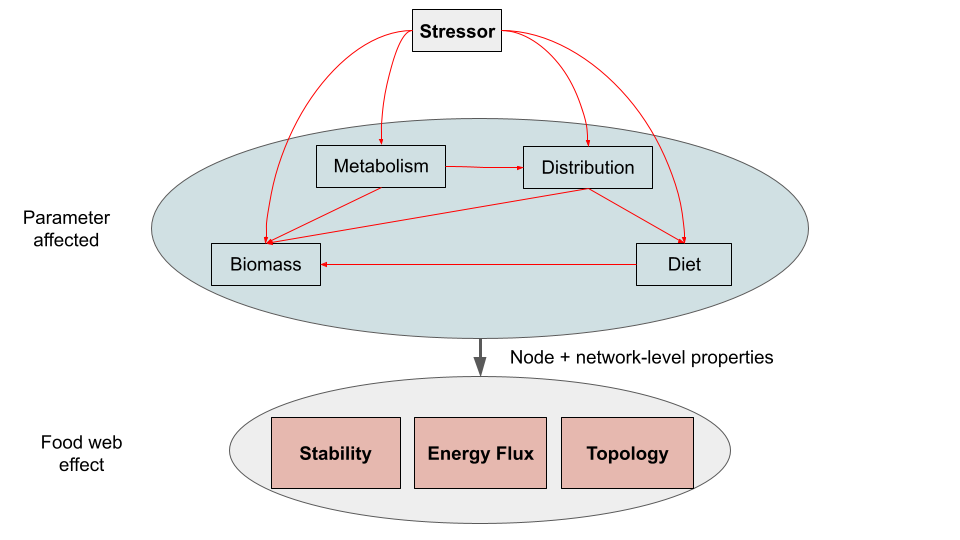
\includegraphics[width=6.27in,height=3.528in]{Figures/Figure2_StressorDiagram.png}
\caption{Conceptual diagram: from species' stressors to food web
effects. See text for explanation.}
\end{figure}

\newpage
\scriptsize

Table 2. Node and network-level properties used to build hypotheses on
the stressors' effects.

\begin{longtable}[]{@{}
  >{\raggedright\arraybackslash}p{(\columnwidth - 6\tabcolsep) * \real{0.1963}}
  >{\raggedright\arraybackslash}p{(\columnwidth - 6\tabcolsep) * \real{0.2617}}
  >{\raggedright\arraybackslash}p{(\columnwidth - 6\tabcolsep) * \real{0.3925}}
  >{\raggedright\arraybackslash}p{(\columnwidth - 6\tabcolsep) * \real{0.1495}}@{}}
\toprule\noalign{}
\begin{minipage}[b]{\linewidth}\raggedright
\textbf{Property}
\end{minipage} & \begin{minipage}[b]{\linewidth}\raggedright
\textbf{Definition}
\end{minipage} & \begin{minipage}[b]{\linewidth}\raggedright
\textbf{Relevance for stressor effects}
\end{minipage} & \begin{minipage}[b]{\linewidth}\raggedright
\textbf{Reference}
\end{minipage} \\
\midrule\noalign{}
\endhead
\bottomrule\noalign{}
\endlastfoot
\emph{Node-level} & & & \\
Degree & Number of feeding interactions in which the species
participates as prey and/or predator. & Perturbations to high-degree
species may have more significant effects on the food web robustness to
perturbations than low-degree species. & Dunne, Williams, \& Martinez
(2002a); Jordán, Benedek, \& Podani (2007) \\
Trophic position & Place in the food web relative to the basal resources
that support the community. Classifies species in: basal, intermediate
and top. & Perturbations on basal resources, intermediate species and
top predators are expected to have large effects on the rest of their
communities if ecosystem control is bottom-up, wasp-waist or top-down,
respectively. & Williams \& Martinez (2000); Thompson, Hemberg,
Starzomski, \& Shurin (2007) \\
Omnivory & Consumer resource use across trophic levels. & High-omnivore
species (generalists) are more flexible than low-omnivore species to
diet changes. & Thompson et al. (2007) \\
Relative abundance & Species' density in proportion to the other species
of the food web. & Perturbations on abundant (dominant) species are
expected to have large effects on the stability and energy flux of the
food and ecosystem, respectively. & Nilsson \& McCann (2016) \\
\emph{Network-level} & & & \\
Conectance & Proportion of actual interactions among possible ones. &
Estimator of community sensitivity to stressors. High connectance gives
resistance and resilience to the food web. & Dunne, Williams, \&
Martinez (2002b) \\
Path length & Average distance, accounted by the number of interactions,
between any pair of species. & Short distances enhance rapid and broad
propagation of perturbations. & Albert \& Barabási (2002) \\
Mean TL & Average of all species' trophic position contained in the food
web. & Influences the magnitude and efficiency of trophic transfer. A
higher mean food chain length reflects increased energy availability and
productivity. & Duffy et al. (2007); Olivier et al. (2019) \\
Omnivory & Proportion of species that feed at different trophic levels.
& It provides trophic flexibility to an ecosystem. Reduces probability
of trophic cascades. & Kratina, LeCraw, Ingram, \& Anholt (2012) \\
\end{longtable}

\normalsize

\hypertarget{main-stressor-effects-in-food-webs-in-a-southwest-atlantic---antarctic-gradient}{%
\subsubsection{4.1 Main stressor effects in food webs in a southwest
Atlantic - Antarctic
gradient}\label{main-stressor-effects-in-food-webs-in-a-southwest-atlantic---antarctic-gradient}}


The most common stressor reported along the southwest Atlantic -
Antarctic gradient is global warming, except for Beagle Channel and
Burdwood Bank, which are more influenced by the introduction of an alien
species and fisheries, respectively (section 3, Table 3). The main
characteristics of global warming in the region, and the most plausible
drivers of change, are: sea warming, glacial retreat, elevated sediment
input in the water column, and reduction of the sea ice extent. These
drivers act in different ways and magnitudes in the studied locations
along the latitudinal gradient. Despite emphasizing global warming in
this section, this does not mean that no other stressors act or interact
with global warming in the study systems, potentially buffering the
overall effect on the food web (e.g.~sea warming and fishery in San
Jorge Gulf). Climate change has led to several well-documented impacts
on marine species regarding distributional shifts induced by warming of
marine currents (Wu et al., 2012; Poloczanska et al., 2013; Vergés et
al., 2019). Furthermore, warmer temperatures increase species metabolic
rates (Brown, Gillooly, Allen, Savage, \& West, 2004). Changes in
metabolic rates can subsequently translate into shifts in species traits
(body size, Vucic-Pestic, Ehnes, Rall, \& Brose (2011); Klein, Hill,
Hinke, Phillips, \& Watters (2018){]}, biomass (Perry et al., 2020) and
distribution (Kortsch, Primicerio, Fossheim, Dolgov, \& Aschan, 2015).
Alterations in the species body size and distributions have ripple
effects on feeding interactions, for example, it can introduce new
feeding interactions (Vergés et al., 2014; Pecuchet et al., 2020),
modify existing ones, and shorten energy pathways (Bartley et al., 2019;
O'Gorman et al., 2019), and reduce trophic efficiencies (Vucic-Pestic et
al., 2011).

In recent years, several new fish (Galván et al., 2022) and
macroinvertebrates species (Vinuesa, 2005; López-Gappa, 2022) were
registered in Patagonia, mostly in San Jorge Gulf in relation to the
southward range shift of warm-temperate species. This distributional
change is driven by the tropicalization of temperate waters caused by
sea warming (Vergés et al., 2014; Vergés et al., 2019). Because of its
location in the ecotone between two biogeographic provinces, the
Argentine (30°S - 44°S) and the Magellanic (43°S - 55°S) (Balech \&
Ehrlich, 2008), the San Jorge Gulf is prone to changes in species
composition. We hypothesize that sea warming will alter the food web
structure topologically, by increasing the number of species and
interactions. Newcomers are, in general, mid-trophic level species with
generalist diets, hence an increase in food web connectance may be
expected (Bartley et al., 2019). In another temperate ecosystem, an
increase in the number of fish species, led to an increase in functional
diversity and predation rate (Sgarlatta, 2023); consequences that may
also be expected in San Jorge Gulf. Given the short path length of the
San Jorge Gulf food web, the disturbances from the listed stressors are
expected to spread to many species of the food web (Table 3). However,
it has to be acknowledged that the increase in functional diversity
driven by the range expansion of warm-temperate species is contrary to
the process of homogenization and loss of functional diversity in the
area driven by trawl fisheries (Rincón-Díaz et al., 2021).

In the middle of the latitudinal gradient (considered in this study),
the Scotia Sea has experienced one of the largest levels of sea warming
of any polar region (Whitehouse et al., 2008; Atkinson et al., 2019).
López-López et al. (2022) suggested that the southward distributional
shift of generalist predators from the northern towards southern Scotia
Sea increases network connectance of the latter, while decreasing its
modularity. The lower modularity may increase the probability of
perturbations spreading through the network (Stouffer \& Bascompte,
2011), which may be offset by increased connectance enhancing robustness
to species loss (Dunne et al., 2002a). In the northern Scotia Sea around
South Georgia Island, we suggest that the declining krill biomass driven
by sea warming (Atkinson et al., 2019), ocean acidification and
pollution synergy (Rowlands et al., 2021), will reduce the energy
transfer to top predators like seabirds and marine mammals. However,
this may be buffered since the dominant copepod species have maintained
their distribution (Tarling et al., 2018), but most importantly, showed
an abundance increase in recent decades likely due to reduced predation
and competition for food (Ward, Tarling, \& Thorpe, 2018). All this is
significant for the structure of the food web given the central role of
krill and copepods, characterized by high degree and mid-trophic
position (Table S1). Overall, the food web's inherent resilience, marked
by high connectance and omnivory, added to the potential compensation
for the krill decrease due to a copepod increase, may buffer against
structural changes (Table 3).

In Potter Cove, a fjord-like Antarctic ecosystem, the impacts of climate
change affect many species within the food web. Potter Cove has recently
experienced frequent events of marine heatwaves, i.e.~prolonged periods
of anomalously high sea surface temperatures (Oliver et al., 2018;
Latorre et al., 2023). This has led to decreases in biomasses of
different planktonic functional groups (Garcia et al., 2019; Latorre et
al., 2023). Given the relatively low abundance of phytoplankton,
zooplankton's low degree, and the modular configuration of the food web,
we hypothesize that changes in these nodes, due to increased sea
temperatures, will be retained in the basal pelagic compartment of the
food web and will not expand to higher trophic levels. Benthic primary
producers in Potter Cove are being influence by the decrease in winter
sea ice cover (higher light availability), the increased levels of
sediments in the water column due to glacial melt run-off (lower light
penetration) and the newly free-ice areas available for colonization
associated to glacier retreat. The overall local effect of climate
change on macroalgae is a net increase in their production (Dolores
Deregibus et al., 2023). It has been proposed that larger diversity in
primary producers can support a more diverse food web with more
specialized consumers (Iken et al., 2023). We expect to see differential
effects of climate change on hard and soft bottom associated food webs
(Cordone et al., 2020). Given the high relative abundance and the high
degree of the macroalgae functional group (Table S1), we expect a longer
hard bottom food web, wider consumer trophic niches, and that it will
become more stable as sea ice cover decreases and the glacier retreats
due to global warming. In soft bottom areas of the Cove, multiple food
web nodes are being affected by ongoing warming effects: decrease in net
primary production of benthic microalgae (Hoffmann et al., 2019), and
changes in the benthic community biomass, distribution and composition
(Pasotti et al., 2015; Sahade et al., 2015). Given that the Potter Cove
food web's present low connectance and omnivory, we suggest fragility
and potential trophic cascade effects (Marina et al., 2018) with
pronounced changes in energy fluxes (Table 3).

The southernmost location of the latitudinal gradient is the Weddell
Sea, where the main effect of global warming is the decrease in sea ice
extent, with reported anomalies in the past summer seasons (Fretwell et
al., 2023). Declining sea ice extent has reduced the abundance of krill
(Atkinson et al., 2004; Flores et al., 2012), and produced an increase
in phytoplankton productivity (Pinkerton et al., 2021; Isla, 2023),
altering the plankton community structure, and benefiting cryptophytes
over diatoms (Lin et al., 2021). Moreover, habitat loss from sea ice
decline will reduce the foraging success and breeding sites of seabirds
(e.g., snow petrel Pagodroma nivea and emperor penguin Aptenodytes
forsteri), decreasing their biomassess and modifying their
distributions. The projected rise in iceberg scouring is expected to
significantly alter the biomass and community structure of macrobenthos,
which in turn will impact mid-trophic level predators such as demersal
fish (Gutt, 2001; Mintenbeck et al., 2012). While we do not anticipate
large-scale topological changes in the food web, local extinctions could
lead to such changes, particularly affecting benthic species (Gutt \&
Piepenburg, 2003). Given that the impacted species---whether
individually like krill, or collectively like macrobenthos---present a
mid-trophic position, high biomass and high degree (Table S1), we
hypothesize that significant shifts in energy fluxes will occur (Table
3). Additionally, the food web's low proportion of omnivores suggests
reduced system resilience (Table 1), increasing the likelihood of regime
changes (Gutt et al., 2015).

The two ecosystems in the subantarctic region, the Beagle Channel and
Burdwood Bank, are more affected by other anthropogenic stressors than
warming. Although these areas are being impacted by sea warming,
potentially affecting vertebrate and invertebrate species (Franco et
al., 2020), to date no studies exist for Beagle Channel and Burdwood
Bank ecosystems. In the Beagle Channel, the introduction of chinook
salmon, a non-native species, poses a significant risk to the existing
food web (Fernández et al., 2010). We hypothesize that chinook salmon's
predation on Fuegian sprat and black southern cod will disrupt the
established patterns of interaction within the food web. Both of these
prey species are crucial for food web dynamics due to their mid-trophic
positions and relatively high abundance (Table S1). Moreover, we expect
that changes in the black southern cod population will have a more
significant impact on the food web than changes in the Fuegian sprat
population, as the black southern cod has a higher degree (Table S1).
Overall, these disruptions could have far-reaching effects on the
ecosystem. This is particularly concerning given the short path length
of the food web, which means that changes can quickly propagate through
the system, affecting many species and potentially destabilizing the
entire network. This phenomenon is further heightened by the ecosystem's
inherent vulnerability to changes at mid-trophic levels, often referred
to as wasp-waist control (Table 3). In the Burdwood Bank region, fishing
activities may be the main stressor causing shifts in the food web
(Table S2). We hypothesize that a combination of factors will
destabilize the already fragile ecosystem, characterized by low
connectance and low omnivory (Table 1). These factors include a decline
in the biomass of the Patagonian toothfish -a key, highly-connected
species (Table S1)- as well as smaller changes in the biomass of four
mid-level fish species, five top-level seabird species, and over 30
types of benthic macroinvertebrates due to bycatch (Gaitán \& Marí,
2016; Martínez et al., 2022; Tamini et al., 2023). Additionally,
alterations in the diets of six seabird species, caused by discarded
catch (Tamini et al., 2023), are expected to disrupt the energy flow and
further reduce the stability of the food web (Table 3).

\scriptsize

Table 3. Summary of food web (FW) effects according to the main
stressors reported for each study area. *Industrial trawl fishery ceased
in 2015 remaining artisanal trawling activity.

\begin{longtable}[]{@{}
  >{\raggedright\arraybackslash}p{(\columnwidth - 4\tabcolsep) * \real{0.3333}}
  >{\raggedright\arraybackslash}p{(\columnwidth - 4\tabcolsep) * \real{0.3194}}
  >{\raggedright\arraybackslash}p{(\columnwidth - 4\tabcolsep) * \real{0.3333}}@{}}
\toprule\noalign{}
\begin{minipage}[b]{\linewidth}\raggedright
\textbf{Study area}
\end{minipage} & \begin{minipage}[b]{\linewidth}\raggedright
\textbf{Stressor}
\end{minipage} & \begin{minipage}[b]{\linewidth}\raggedright
\textbf{Food web effects}
\end{minipage} \\
\midrule\noalign{}
\endhead
\bottomrule\noalign{}
\endlastfoot
\textbf{San Jorge Gulf} & & \\
& Fishery* & ↑ FW connectance

↓ FW stability

↓ functional diversity \\
& Sea warming & Shifts in FW topology

↑ FW connectance

↑ functional diversity \\
\textbf{Beagle Channel} & & \\
& Alien species & Shifts in FW topology

↑ spread of perturbations \\
\textbf{Burdwood Bank} & & \\
& Fishery & Shifts in main energy fluxes

↓ FW stability \\
\textbf{Scotia Sea} & & \\
& Sea warming & ↑ FW connectance

↓ FW modularity

↓ energy transfer to high TLs

↑ spread of perturbation \\
\textbf{Potter Cove (Antarctica)} & & \\
& Sea warming & ↓ perturbation spreading \\
& Sea ice decline + glacial retreat & Differential impacts, by
substrate: hard (HS) or soft (SS)

↑ FW chain length \& ↑ trophic niches (HS)

↑ FW fragility \& trophic cascades (SS) \\
\textbf{Weddell Sea (Antarctica)} & & \\
& Sea ice decline + iceberg scouring & Shifts in main energy fluxes

↑ likelihood of regime shifts

↓ resilience \\
\end{longtable}

\normalsize

\hypertarget{gaps-and-future-perspectives}{%
\subsection{5. Gaps and future
perspectives}\label{gaps-and-future-perspectives}}

In the selected study areas along the southwest Atlantic to Antarctic
latitudinal gradient, several stressors may directly affect consumers'
diets triggered by modified environmental conditions (sea warming,
reduced sea ice extent) and new species (due to species' distributional
shifts and introductions). Moreover, the population trends (biomasses
and abundances) of important species are also changing (Hindell et al.,
2020; Funes, 2020; Woods et al., 2023) driving shifts in their roles as
either predators or prey (e.g. Belleggia, Giberto, \& Bremec (2017),
Pasti et al. (2021)). These diet and biomass shifts should be
investigated in order to generate reliable predictions of food web
responses to multiple stressors in the southwest Atlantic - Antarctic
region. One could argue that both shifts might increase the complexity
of food webs in the short term by adding generalist predators or new
prey (e.g., Cordone, Galván, \& Momo (2023)) or by enabling discard
consumption (e.g. Funes et al. (2022)). However, in the long term, both
stressors may lead to the biological extinction of certain prey and
competitors (e.g. Anton et al. (2019)) or a significant reduction in
target and incidental catch species (e.g. Dulvy et al. (2014)), thereby
promoting food web simplification.

Since this review deals with qualitative data of prey-predator
interactions and stressor effects influencing them, adding quantitative
data to the food webs (i.e.~interaction strength) and to the stressors
(i.e.~magnitude) would lead to a better comprehension of how a given
stressor acts on specific species which might translate into food web
effects. In this context, it would be useful to develop quantitative
food web models where the strength of interactions reflect energy fluxes
among species (Nilsson \& McCann, 2016; Kortsch et al., 2021). Emerging
methods such as bioenergetic food web modeling have been proposed in
this regard and present promising ways to estimate shifts in species
interactions within food webs as a response to stressors (Gauzens,
Brose, Delmas, \& Berti, n.d.; Gellner, McCann, \& Hastings, 2023).
Shifts that can lead to changes in overall ecosystem functioning and
stability.

Regarding knowledge and data gaps on species and their stressors,
especially the Beagle Channel and Burdwood Bank are poorly sampled study
regions. Almost no information exists on the impact of global warming
effects (sea warming, glacial retreat, ocean acidification) on
communities in these ecosystems, though warming of mid-water and bottom
layers have been shown at a regional scale (Franco et al., 2020). Yet in
Beagle Channel recent experimental studies have tested the tolerance of
fishes to scenarios of sea warming and/or acidification suggesting
potential metabolic impacts on species (María Eugenia Lattuca, Boy,
Vanella, Barrantes, \& Fernández, 2018; María E. Lattuca et al., 2023).

Analyzing the impact of multiple stressors through observational studies
is challenging (Gutt et al., 2021). This complexity arises partly
because of potential for antagonistic effects, where impacts cancel each
other out, or synergistic effects, where the combined impact is greater
than the sum of individual effects (Boyd, Lennartz, Glover, \& Doney,
2015; Côté et al., 2016). Moreover, these interactive effects are
complicated to handle in the framework of complex food webs. The number
of pathways through which a species may affect or be affected by other
species, and through which stressors may permeate communities, increases
exponentially with the number of species and interactions in a network
(Menge, 1995). To tackle this complexity, Beauchesne, Cazelles,
Archambault, Dee, \& Gravel (2021) developed a theory-grounded approach
using motifs (i.e.~groups of species that, when put together, construct
whole food webs) to simplify food webs; a methodology that could be
applied to our food web study cases.

\hypertarget{conclusions}{%
\subsection{Conclusions}\label{conclusions}}

We have reviewed the main environmental and anthropogenic stressors
acting in six different areas along a large-scale latitudinal gradient,
from temperate Atlantic to cold Antarctic ecosystems. Using a
theoretical framework that combines species and food web level data, we
suggest how warming effects may impact food web structure and
functioning. These qualitative predictions are intended to serve as the
basis for future studies in marine ecosystems of the Southern Hemisphere
that aim at quantifying the magnitude of these stressors and how they
are affecting quantitative food web properties, such as energy fluxes
and stability. There is an urgent need to assess these changes using a
holistic and quantitative framework where the magnitude of stressors and
species interactions are taken into account.

\hypertarget{acknowledgements}{%
\subsection{Acknowledgements}\label{acknowledgements}}

This review is a product of the project ``¿Cuáles son los efectos de los
cambios ambientales antropogénicos en las interacciones tróficas de las
comunidades de los ecosistemas marinos en el gradiente latitudinal
Atlántico Sudoccidental - Antártida?'', funded by Consejo Nacional de
Investigaciones Científicas (CONICET, code PIP 2022-2024 \#0907).

\hypertarget{references}{%
\subsection*{References}\label{references}}
\addcontentsline{toc}{subsection}{References}

\hypertarget{refs}{}
\begin{CSLReferences}{1}{0}
\leavevmode\vadjust pre{\hypertarget{ref-Acha2004}{}}%
Acha, E. M., Mianzan, H. W., Guerrero, R. A., Favero, M., \& Bava, J.
(2004). Marine fronts at the continental shelves of austral {South
America}: {Physical} and ecological processes. \emph{Journal of Marine
Systems}, \emph{44}(1), 83--105.
doi:\href{https://doi.org/10.1016/j.jmarsys.2003.09.005}{10.1016/j.jmarsys.2003.09.005}

\leavevmode\vadjust pre{\hypertarget{ref-APN2022}{}}%
Administración de Parques Nacionales. (2022). {Plan de gestión AMP
Namuncurá Banco Burdwood}. {Dirección Nacional de Áreas Marinas
Protegidas (DNAMP), Argentina}.

\leavevmode\vadjust pre{\hypertarget{ref-Albert2002}{}}%
Albert, R., \& Barabási, A.-L. (2002). Statistical mechanics of complex
networks. \emph{Reviews of Modern Physics}, \emph{74}(1), 47--97.
doi:\href{https://doi.org/10.1103/RevModPhys.74.47}{10.1103/RevModPhys.74.47}

\leavevmode\vadjust pre{\hypertarget{ref-Allega2019}{}}%
Allega, Lucrecia, Braverman, M. S., Cabreira, A. G., Campodónico, S.,
Colonello, J. H., Derisio, C. M., \ldots{} Verón, E. M. (2019).
\emph{{Estado del conocimiento biológico pesquero de los principales
recursos vivos y su ambiente, con relación a la exploración
hidrocarburífera en la Zona Económica Exclusiva Argentina y
adyacencias}}. {INIDEP}.

\leavevmode\vadjust pre{\hypertarget{ref-Allega2020}{}}%
Allega, L., Braverman, M., Campodónico, S., Carozza, C. R., Cepeda, G.
D., Colonello, J. H., \ldots{} Verón, E. (2020). \emph{{Estado del
conocimiento biológico pesquero de los principales recursos vivos y su
ambiente, con relación a la exploración hidrocarburífera en la Zona
Económica Exclusiva argentina y sus adyacencias}}. {Mar del Plata}:
{Instituto Nacional de Investigación y Desarrollo Pesquero (INIDEP)}.

\leavevmode\vadjust pre{\hypertarget{ref-Anton2019}{}}%
Anton, A., Geraldi, N. R., Lovelock, C. E., Apostolaki, E. T., Bennett,
S., Cebrian, J., \ldots{} Duarte, C. M. (2019). Global ecological
impacts of marine exotic species. \emph{Nature Ecology \& Evolution},
\emph{3}(5), 787--800.
doi:\href{https://doi.org/10.1038/s41559-019-0851-0}{10.1038/s41559-019-0851-0}

\leavevmode\vadjust pre{\hypertarget{ref-Antoni2020}{}}%
Antoni, J. S., Almandoz, G. O., Ferrario, M. E., Hernando, M. P.,
Varela, D. E., Rozema, P. D., \ldots{} Schloss, I. R. (2020). Response
of a natural {Antarctic} phytoplankton assemblage to changes in
temperature and salinity. \emph{Journal of Experimental Marine Biology
and Ecology}, \emph{532}, 151444.
doi:\href{https://doi.org/10.1016/j.jembe.2020.151444}{10.1016/j.jembe.2020.151444}

\leavevmode\vadjust pre{\hypertarget{ref-Atkinson2019}{}}%
Atkinson, A., Hill, S. L., Pakhomov, E. A., Siegel, V., Reiss, C. S.,
Loeb, V. J., \ldots{} Sailley, S. F. (2019). Krill ({Euphausia} superba)
distribution contracts southward during rapid regional warming.
\emph{Nature Climate Change}, \emph{9}(2), 142--147.
doi:\href{https://doi.org/10.1038/s41558-018-0370-z}{10.1038/s41558-018-0370-z}

\leavevmode\vadjust pre{\hypertarget{ref-Atkinson2004}{}}%
Atkinson, A., Siegel, V., Pakhomov, E., \& Rothery, P. (2004). Long-term
decline in krill stock and increase in salps within the {Southern
Ocean}. \emph{Nature}, \emph{432}(7013), 100--103.
doi:\href{https://doi.org/10.1038/nature02996}{10.1038/nature02996}

\leavevmode\vadjust pre{\hypertarget{ref-Balech2008}{}}%
Balech, E., \& Ehrlich, M. D. (2008). {Esquema biogeográfico del Mar
Argentino}.

\leavevmode\vadjust pre{\hypertarget{ref-Bartley2019}{}}%
Bartley, T. J., McCann, K. S., Bieg, C., Cazelles, K., Granados, M.,
Guzzo, M. M., \ldots{} McMeans, B. C. (2019). Food web rewiring in a
changing world. \emph{Nature Ecology \& Evolution}, \emph{3}(3),
345--354.
doi:\href{https://doi.org/10.1038/s41559-018-0772-3}{10.1038/s41559-018-0772-3}

\leavevmode\vadjust pre{\hypertarget{ref-Bauer2022}{}}%
Bauer, B., Berti, E., Ryser, R., Gauzens, B., Hirt, M. R., Rosenbaum,
B., \ldots{} Brose, U. (2022). Biotic filtering by species' interactions
constrains food-web variability across spatial and abiotic gradients.
\emph{Ecology Letters}, \emph{25}(5), 1225--1236.
doi:\href{https://doi.org/10.1111/ele.13995}{10.1111/ele.13995}

\leavevmode\vadjust pre{\hypertarget{ref-Beauchesne2021}{}}%
Beauchesne, D., Cazelles, K., Archambault, P., Dee, L. E., \& Gravel, D.
(2021). On the sensitivity of food webs to multiple stressors.
\emph{Ecology Letters}, \emph{24}(10), 2219--2237.
doi:\href{https://doi.org/10.1111/ele.13841}{10.1111/ele.13841}

\leavevmode\vadjust pre{\hypertarget{ref-Belgrano2005}{}}%
Belgrano, A., Scharler, S. E. R. C. U. M., Scharler, U. M., Dunne, J.,
\& Ulanowicz, R. E. (2005). \emph{Aquatic {Food Webs}: {An Ecosystem
Approach}}. {OUP Oxford}.

\leavevmode\vadjust pre{\hypertarget{ref-Belleggia2017}{}}%
Belleggia, M., Giberto, D., \& Bremec, C. (2017). Adaptation of diet in
a changed environment: {Increased} consumption of lobster krill {Munida}
gregaria ({Fabricius}, 1793) by {Argentine} hake. \emph{Marine Ecology},
\emph{38}(4), e12445.
doi:\href{https://doi.org/10.1111/maec.12445}{10.1111/maec.12445}

\leavevmode\vadjust pre{\hypertarget{ref-Bovcon2013}{}}%
Bovcon, N. D., Góngora, M. E., Marinao, C., \& González-Zevallos, D.
(2013). Composición de las capturas y descartes generados en la pesca de
merluza común {Merluccius} hubbsi y langostino patagónico {Pleoticus}
muelleri: Un caso de estudio en la flota fresquera de altura del {Golfo
San Jorge}, {Chubut}, {Argentina}. \emph{Revista de Biología Marina y
Oceanografía}, \emph{48}(2), 303--319.
doi:\href{https://doi.org/10.4067/S0718-19572013000200010}{10.4067/S0718-19572013000200010}

\leavevmode\vadjust pre{\hypertarget{ref-Boyd2015}{}}%
Boyd, P. W., Lennartz, S. T., Glover, D. M., \& Doney, S. C. (2015).
Biological ramifications of climate-change-mediated oceanic
multi-stressors. \emph{Nature Climate Change}, \emph{5}(1), 71--79.
doi:\href{https://doi.org/10.1038/nclimate2441}{10.1038/nclimate2441}

\leavevmode\vadjust pre{\hypertarget{ref-Braeckman2021}{}}%
Braeckman, U., Pasotti, F., Hoffmann, R., Vázquez, S., Wulff, A.,
Schloss, I. R., \ldots{} Vanreusel, A. (2021). Glacial melt disturbance
shifts community metabolism of an {Antarctic} seafloor ecosystem from
net autotrophy to heterotrophy. \emph{Communications Biology},
\emph{4}(1), 148.
doi:\href{https://doi.org/10.1038/s42003-021-01673-6}{10.1038/s42003-021-01673-6}

\leavevmode\vadjust pre{\hypertarget{ref-Braithwaite2015}{}}%
Braithwaite, J. E., Meeuwig, J. J., Letessier, T. B., Jenner, K. C. S.,
\& Brierley, A. S. (2015). From sea ice to blubber: Linking whale
condition to krill abundance using historical whaling records.
\emph{Polar Biology}, \emph{38}(8), 1195--1202.
doi:\href{https://doi.org/10.1007/s00300-015-1685-0}{10.1007/s00300-015-1685-0}

\leavevmode\vadjust pre{\hypertarget{ref-Brown2004}{}}%
Brown, J. H., Gillooly, J. F., Allen, A. P., Savage, V. M., \& West, G.
B. (2004). Toward a {Metabolic Theory} of {Ecology}. \emph{Ecology},
\emph{85}(7), 1771--1789.
doi:\href{https://doi.org/10.1890/03-9000}{10.1890/03-9000}

\leavevmode\vadjust pre{\hypertarget{ref-Bruder2019}{}}%
Bruder, A., Frainer, A., Rota, T., \& Primicerio, R. (2019). The
{Importance} of {Ecological Networks} in {Multiple-Stressor Research}
and {Management}. \emph{Frontiers in Environmental Science}, \emph{7}.

\leavevmode\vadjust pre{\hypertarget{ref-Bruno2023}{}}%
Bruno, D. O., Riccialdelli, L., Acha, E. M., \& Fernández, D. A. (2023).
Seasonal variation of autochthonous and allochthonous carbon sources for
the first levels of the {Beagle Channel} food web. \emph{Journal of
Marine Systems}, \emph{239}, 103859.
doi:\href{https://doi.org/10.1016/j.jmarsys.2023.103859}{10.1016/j.jmarsys.2023.103859}

\leavevmode\vadjust pre{\hypertarget{ref-Chown2022}{}}%
Chown, S. L., Leihy, R. I., Naish, T. R., Brooks, C. M., Convey, P.,
Henley, B. J., \ldots{} Grant, S. M. (2022). Antarctic climate change
and the environment: A decadal synopsis and recommendations for action.

\leavevmode\vadjust pre{\hypertarget{ref-Ciancio2008}{}}%
Ciancio, J. E., Pascual, M. A., Botto, F., Frere, E., \& Iribarne, O.
(2008). Trophic relationships of exotic anadromous salmonids in the
southern {Patagonian Shelf} as inferred from stable isotopes.
\emph{Limnology and Oceanography}, \emph{53}(2), 788--798.
doi:\href{https://doi.org/10.4319/lo.2008.53.2.0788}{10.4319/lo.2008.53.2.0788}

\leavevmode\vadjust pre{\hypertarget{ref-Cirtwill2015}{}}%
Cirtwill, A. R., Stouffer, D. B., \& Romanuk, T. N. (2015). Latitudinal
gradients in biotic niche breadth vary across ecosystem types.
\emph{Proceedings of the Royal Society B: Biological Sciences},
\emph{282}(1819), 20151589.
doi:\href{https://doi.org/10.1098/rspb.2015.1589}{10.1098/rspb.2015.1589}

\leavevmode\vadjust pre{\hypertarget{ref-Collins2010}{}}%
Collins, M. A., Brickle, P., Brown, J., \& Belchier, M. (2010). Chapter
{Four} - {The Patagonian Toothfish}: {Biology}, {Ecology} and {Fishery}.
In M. Lesser (Ed.), \emph{Advances in {Marine Biology}} (Vol. 58, pp.
227--300). {Academic Press}.
doi:\href{https://doi.org/10.1016/B978-0-12-381015-1.00004-6}{10.1016/B978-0-12-381015-1.00004-6}

\leavevmode\vadjust pre{\hypertarget{ref-Commendatore2012}{}}%
Commendatore, M. G., Nievas, M. L., Amin, O., \& Esteves, J. L. (2012).
Sources and distribution of aliphatic and polyaromatic hydrocarbons in
coastal sediments from the {Ushuaia Bay} ({Tierra} del {Fuego},
{Patagonia}, {Argentina}). \emph{Marine Environmental Research},
\emph{74}, 20--31.
doi:\href{https://doi.org/10.1016/j.marenvres.2011.11.010}{10.1016/j.marenvres.2011.11.010}

\leavevmode\vadjust pre{\hypertarget{ref-Constable2014}{}}%
Constable, A. J., Melbourne-Thomas, J., Corney, S. P., Arrigo, K. R.,
Barbraud, C., Barnes, D. K. A., \ldots{} Ziegler, P. (2014). Climate
change and {Southern Ocean} ecosystems {I}: How changes in physical
habitats directly affect marine biota. \emph{Global Change Biology},
\emph{20}(10), 3004--3025.
doi:\href{https://doi.org/10.1111/gcb.12623}{10.1111/gcb.12623}

\leavevmode\vadjust pre{\hypertarget{ref-Cordone2023}{}}%
Cordone, G., Galván, D. E., \& Momo, F. R. (2023). Impacts of an
invasion by green crab {Carcinus} maenas on the intertidal food web of a
{Patagonian} rocky shore, {Argentina}. \emph{Marine Ecology Progress
Series}, \emph{713}, 97--115.
doi:\href{https://doi.org/10.3354/meps14336}{10.3354/meps14336}

\leavevmode\vadjust pre{\hypertarget{ref-Cordone2020}{}}%
Cordone, G., Salinas, V., Marina, T. I., Doyle, S. R., Pasotti, F.,
Saravia, L. A., \& Momo, F. R. (2020). Green vs brown food web:
{Effects} of habitat type on multidimensional stability proxies for a
highly-resolved {Antarctic} food web. \emph{Food Webs}, \emph{25},
e00166.
doi:\href{https://doi.org/10.1016/j.fooweb.2020.e00166}{10.1016/j.fooweb.2020.e00166}

\leavevmode\vadjust pre{\hypertarget{ref-Correa2008}{}}%
Correa, C., \& Gross, M. R. (2008). Chinook salmon invade southern
{South America}. \emph{Biological Invasions}, \emph{10}(5), 615--639.
doi:\href{https://doi.org/10.1007/s10530-007-9157-2}{10.1007/s10530-007-9157-2}

\leavevmode\vadjust pre{\hypertarget{ref-Cossi2021}{}}%
Cossi, P. F., Ojeda, M., Chiesa, I. L., Rimondino, G. N., Fraysse, C.,
Calcagno, J., \& Pérez, A. F. (2021). First evidence of microplastics in
the {Marine Protected Area Namuncurá} at {Burdwood Bank}, {Argentina}: A
study on {Henricia} obesa and {Odontaster} penicillatus
({Echinodermata}: {Asteroidea}). \emph{Polar Biology}, \emph{44}(12),
2277--2287.
doi:\href{https://doi.org/10.1007/s00300-021-02959-5}{10.1007/s00300-021-02959-5}

\leavevmode\vadjust pre{\hypertarget{ref-Cote2016}{}}%
Côté, I. M., Darling, E. S., \& Brown, C. J. (2016). Interactions among
ecosystem stressors and their importance in conservation.
\emph{Proceedings of the Royal Society B: Biological Sciences},
\emph{283}(1824), 20152592.
doi:\href{https://doi.org/10.1098/rspb.2015.2592}{10.1098/rspb.2015.2592}

\leavevmode\vadjust pre{\hypertarget{ref-deHaro2022}{}}%
de Haro, J. C., Perez Orsi, H., Cané, S., Di Pangracio, A., Falabella,
V., \& Sapoznikow, A. (2022). {Informe colaborativo sobre el Estado de
situación. Riesgos e impactos de la prospección sísmica en el Mar
Argentino}. {Foro para la Conservación del Mar Patagónico y Áreas de
Influencia}.

\leavevmode\vadjust pre{\hypertarget{ref-Deregibus2023}{}}%
Deregibus, Dolores, Campana, G. L., Neder, C., Barnes, D. K. A., Zacher,
K., Piscicelli, J. M., \ldots{} Quartino, M. L. (2023). Potential
macroalgal expansion and blue carbon gains with northern {Antarctic
Peninsula} glacial retreat. \emph{Marine Environmental Research},
\emph{189}, 106056.
doi:\href{https://doi.org/10.1016/j.marenvres.2023.106056}{10.1016/j.marenvres.2023.106056}

\leavevmode\vadjust pre{\hypertarget{ref-Deregibus2017}{}}%
Deregibus, D., Quartino, M. L., Zacher, K., Campana, G. L., \& Barnes,
D. K. A. (2017). Understanding the link between sea ice, ice scour and
{Antarctic} benthic biodiversity\textendash the need for cross-station
and international collaboration. \emph{Polar Record}, \emph{53}(2),
143--152.
doi:\href{https://doi.org/10.1017/S0032247416000875}{10.1017/S0032247416000875}

\leavevmode\vadjust pre{\hypertarget{ref-Deregibus2020}{}}%
Deregibus, Dolores, Zacher, K., Bartsch, I., Campana, G. L., Momo, F.
R., Wiencke, C., \ldots{} Quartino, M. L. (2020). Carbon {Balance Under}
a {Changing Light Environment}. In I. Gómez \& P. Huovinen (Eds.),
\emph{Antarctic {Seaweeds}: {Diversity}, {Adaptation} and {Ecosystem
Services}} (pp. 173--191). {Cham}: {Springer International Publishing}.
doi:\href{https://doi.org/10.1007/978-3-030-39448-6_9}{10.1007/978-3-030-39448-6\_9}

\leavevmode\vadjust pre{\hypertarget{ref-DiMauro2022}{}}%
Di Mauro, R., Castillo, S., Pérez, A., Iachetti, C. M., Silva, L.,
Tomba, J. P., \& Chiesa, I. L. (2022). Anthropogenic microfibers are
highly abundant at the {Burdwood Bank} seamount, a protected
sub-{Antarctic} environment in the {Southwestern Atlantic Ocean}.
\emph{Environmental Pollution}, \emph{306}, 119364.
doi:\href{https://doi.org/10.1016/j.envpol.2022.119364}{10.1016/j.envpol.2022.119364}

\leavevmode\vadjust pre{\hypertarget{ref-Dodino2022}{}}%
Dodino, S., Riccialdelli, L., Polito, M. J., Pütz, K., Brasso, R. L., \&
Raya Rey, A. (2022). Mercury exposure driven by geographic and trophic
factors in {Magellanic} penguins from {Tierra} del {Fuego}. \emph{Marine
Pollution Bulletin}, \emph{174}, 113184.
doi:\href{https://doi.org/10.1016/j.marpolbul.2021.113184}{10.1016/j.marpolbul.2021.113184}

\leavevmode\vadjust pre{\hypertarget{ref-Duarte2011}{}}%
Duarte, C. A., Giarratano, E., Amin, O. A., \& Comoglio, L. I. (2011).
Heavy metal concentrations and biomarkers of oxidative stress in native
mussels ({Mytilus} edulis chilensis) from {Beagle Channel} coast
({Tierra} del {Fuego}, {Argentina}). \emph{Marine Pollution Bulletin},
\emph{62}(8), 1895--1904.
doi:\href{https://doi.org/10.1016/j.marpolbul.2011.05.031}{10.1016/j.marpolbul.2011.05.031}

\leavevmode\vadjust pre{\hypertarget{ref-Duffy2007}{}}%
Duffy, J. E., Cardinale, B. J., France, K. E., McIntyre, P. B.,
Thébault, E., \& Loreau, M. (2007). The functional role of biodiversity
in ecosystems: Incorporating trophic complexity. \emph{Ecology Letters},
\emph{10}(6), 522--538.
doi:\href{https://doi.org/10.1111/j.1461-0248.2007.01037.x}{10.1111/j.1461-0248.2007.01037.x}

\leavevmode\vadjust pre{\hypertarget{ref-Dulvy2014}{}}%
Dulvy, N. K., Fowler, S. L., Musick, J. A., Cavanagh, R. D., Kyne, P.
M., Harrison, L. R., \ldots{} White, W. T. (2014). Extinction risk and
conservation of the world's sharks and rays. \emph{eLife}, \emph{3},
e00590.
doi:\href{https://doi.org/10.7554/eLife.00590}{10.7554/eLife.00590}

\leavevmode\vadjust pre{\hypertarget{ref-Dunne2002a}{}}%
Dunne, J. A., Williams, R. J., \& Martinez, N. D. (2002a). Food-web
structure and network theory: {The} role of connectance and size.
\emph{Proceedings of the National Academy of Sciences}, \emph{99}(20),
12917--12922.
doi:\href{https://doi.org/10.1073/pnas.192407699}{10.1073/pnas.192407699}

\leavevmode\vadjust pre{\hypertarget{ref-Dunne2002}{}}%
Dunne, J. A., Williams, R. J., \& Martinez, N. D. (2002b). Network
structure and biodiversity loss in food webs: Robustness increases with
connectance. \emph{Ecology Letters}, \emph{5}(4), 558--567.
doi:\href{https://doi.org/10.1046/j.1461-0248.2002.00354.x}{10.1046/j.1461-0248.2002.00354.x}

\leavevmode\vadjust pre{\hypertarget{ref-Fernandez2010}{}}%
Fernández, D. A., Ciancio, J., Ceballos, S. G., Riva-Rossi, C., \&
Pascual, M. A. (2010). Chinook salmon ({Oncorhynchus} tshawytscha,
{Walbaum} 1792) in the {Beagle Channel}, {Tierra} del {Fuego}: The onset
of an invasion. \emph{Biological Invasions}, \emph{12}(9), 2991--2997.
doi:\href{https://doi.org/10.1007/s10530-010-9731-x}{10.1007/s10530-010-9731-x}

\leavevmode\vadjust pre{\hypertarget{ref-Ferreira2021}{}}%
Ferreira, M. F., Lo Nostro, F. L., Fernández, D. A., \& Genovese, G.
(2021). Endocrine disruption in the sub {Antarctic} fish
{Patagonotothen} tessellata ({Perciformes}, {Notothenidae}) from {Beagle
Channel} associated to anthropogenic impact. \emph{Marine Environmental
Research}, \emph{171}, 105478.
doi:\href{https://doi.org/10.1016/j.marenvres.2021.105478}{10.1016/j.marenvres.2021.105478}

\leavevmode\vadjust pre{\hypertarget{ref-Fioramonti2022}{}}%
Fioramonti, N. E., Ribeiro Guevara, S., Becker, Y. A., \& Riccialdelli,
L. (2022). Mercury transfer in coastal and oceanic food webs from the
{Southwest Atlantic Ocean}. \emph{Marine Pollution Bulletin},
\emph{175}, 113365.
doi:\href{https://doi.org/10.1016/j.marpolbul.2022.113365}{10.1016/j.marpolbul.2022.113365}

\leavevmode\vadjust pre{\hypertarget{ref-Flores2012}{}}%
Flores, H., Atkinson, A., Kawaguchi, S., Krafft, B., Milinevsky, G.,
Nicol, S., \ldots{} Werner, T. (2012). Impact of climate change on
{Antarctic} krill. \emph{Marine Ecology Progress Series}, \emph{458},
1--19. doi:\href{https://doi.org/10.3354/meps09831}{10.3354/meps09831}

\leavevmode\vadjust pre{\hypertarget{ref-Franco2020}{}}%
Franco, B. C., Combes, V., \& González Carman, V. (2020). Subsurface
{Ocean Warming Hotspots} and {Potential Impacts} on {Marine Species}:
{The Southwest South Atlantic Ocean Case Study}. \emph{Frontiers in
Marine Science}, \emph{7}.

\leavevmode\vadjust pre{\hypertarget{ref-Fretwell2023}{}}%
Fretwell, P. T., Boutet, A., \& Ratcliffe, N. (2023). Record low 2022
{Antarctic} sea ice led to catastrophic breeding failure of emperor
penguins. \emph{Communications Earth \& Environment}, \emph{4}(1), 1--6.
doi:\href{https://doi.org/10.1038/s43247-023-00927-x}{10.1038/s43247-023-00927-x}

\leavevmode\vadjust pre{\hypertarget{ref-Fuentes2016}{}}%
Fuentes, V., Alurralde, G., Meyer, B., Aguirre, G. E., Canepa, A.,
Wölfl, A.-C., \ldots{} Schloss, I. R. (2016). Glacial melting: An
overlooked threat to {Antarctic} krill. \emph{Scientific Reports},
\emph{6}(1), 27234.
doi:\href{https://doi.org/10.1038/srep27234}{10.1038/srep27234}

\leavevmode\vadjust pre{\hypertarget{ref-Funes2020}{}}%
Funes, M. (2020, March). \emph{Efectos de la pesca de arrastre sobre la
estructura trófica del norte del {Golfo San Jorge}} (PhD thesis).

\leavevmode\vadjust pre{\hypertarget{ref-Funes2019}{}}%
Funes, M., Marinao, C., \& Galván, D. E. (2019). Does trawl fisheries
affect the diet of fishes? {A} stable isotope analysis approach*.
\emph{Isotopes in Environmental and Health Studies}, \emph{55}(4),
327--343.
doi:\href{https://doi.org/10.1080/10256016.2019.1626381}{10.1080/10256016.2019.1626381}

\leavevmode\vadjust pre{\hypertarget{ref-Funes2022}{}}%
Funes, M., Saravia, L. A., Cordone, G., Iribarne, O. O., \& Galván, D.
E. (2022). Network analysis suggests changes in food web stability
produced by bottom trawl fishery in {Patagonia}. \emph{Scientific
Reports}, \emph{12}(1), 10876.
doi:\href{https://doi.org/10.1038/s41598-022-14363-y}{10.1038/s41598-022-14363-y}

\leavevmode\vadjust pre{\hypertarget{ref-Gaitan2016}{}}%
Gaitán, E., \& Marí, N. (2016). {Análisis de las comunidades bentónicas
asociadas a capturas de la flota comercial dirigida a Macruronus
magellanicus}. {Instituto Nacional de Investigación y Desarrollo
Pesquero (INIDEP)}.

\leavevmode\vadjust pre{\hypertarget{ref-Galvan2022}{}}%
Galván, D. E., Bovcon, N. D., Cochia, P. D., González, R. A., Lattuca,
M. E., Reinaldo, M. O., \ldots{} Svendsen, G. M. (2022). Changes in the
{Specific} and {Biogeographic Composition} of {Coastal Fish Assemblages}
in {Patagonia}, {Driven} by {Climate Change}, {Fishing}, and {Invasion}
by {Alien Species}. In E. W. Helbling, M. A. Narvarte, R. A. González,
\& V. E. Villafañe (Eds.), \emph{Global {Change} in {Atlantic Coastal
Patagonian Ecosystems}: {A Journey Through Time}} (pp. 205--231).
{Cham}: {Springer International Publishing}.
doi:\href{https://doi.org/10.1007/978-3-030-86676-1_9}{10.1007/978-3-030-86676-1\_9}

\leavevmode\vadjust pre{\hypertarget{ref-Garcia2019}{}}%
Garcia, M. D., Fernández Severini, M. D., Spetter, C., López Abbate, M.
C., Tartara, M. N., Nahuelhual, E. G., \ldots{} Hoffmeyer, M. S. (2019).
Effects of glacier melting on the planktonic communities of two
{Antarctic} coastal areas ({Potter Cove} and {Hope Bay}) in summer.
\emph{Regional Studies in Marine Science}, \emph{30}, 100731.
doi:\href{https://doi.org/10.1016/j.rsma.2019.100731}{10.1016/j.rsma.2019.100731}

\leavevmode\vadjust pre{\hypertarget{ref-Garcia2016}{}}%
Garcia, M. D., Hoffmeyer, M. S., Abbate, M. C. L., Barría De Cao, M. S.,
Pettigrosso, R. E., Almandoz, G. O., \ldots{} Schloss, I. R. (2016).
Micro- and mesozooplankton responses during two contrasting summers in a
coastal {Antarctic} environment. \emph{Polar Biology}, \emph{39}(1),
123--137.
doi:\href{https://doi.org/10.1007/s00300-015-1678-z}{10.1007/s00300-015-1678-z}

\leavevmode\vadjust pre{\hypertarget{ref-Garcia-Borboroglu2008}{}}%
García-Borboroglu, P., Boersma, P. D., Reyes, L., \& Skewgar, E. (2008).
Petroleum {Pollution} and {Penguins}: {Marine Conservation Tools} to
{Reduce} the {Problem}. In \emph{Marine {Pollution}: {New} research}
(Hofer, T.N., pp. 339--356). {New York, USA}: {Nova Science Publishers
Inc.}

\leavevmode\vadjust pre{\hypertarget{ref-Gauzens2023}{}}%
Gauzens, B., Brose, U., Delmas, E., \& Berti, E. (n.d.). {ATNr}:
{Allometric Trophic Network} models in {R}. \emph{Methods in Ecology and
Evolution}, \emph{n/a}(n/a).
doi:\href{https://doi.org/10.1111/2041-210X.14212}{10.1111/2041-210X.14212}

\leavevmode\vadjust pre{\hypertarget{ref-Gellner2023}{}}%
Gellner, G., McCann, K., \& Hastings, A. (2023). Stable diverse food
webs become more common when interactions are more biologically
constrained. \emph{Proceedings of the National Academy of Sciences},
\emph{120}(31), e2212061120.
doi:\href{https://doi.org/10.1073/pnas.2212061120}{10.1073/pnas.2212061120}

\leavevmode\vadjust pre{\hypertarget{ref-Gil2011}{}}%
Gil, M. N., Torres, A. I., Amin, O., \& Esteves, J. L. (2011).
Assessment of recent sediment influence in an urban polluted
subantarctic coastal ecosystem. {Beagle Channel} ({Southern Argentina}).
\emph{Marine Pollution Bulletin}, \emph{62}(1), 201--207.
doi:\href{https://doi.org/10.1016/j.marpolbul.2010.10.004}{10.1016/j.marpolbul.2010.10.004}

\leavevmode\vadjust pre{\hypertarget{ref-Glembocki2015}{}}%
Glembocki, N. G., Williams, G. N., Góngora, M. E., Gagliardini, D. A.,
\& Orensanz, J. M. (Lobo). (2015). Synoptic oceanography of {San Jorge
Gulf} ({Argentina}): {A} template for {Patagonian} red shrimp
({Pleoticus} muelleri) spatial dynamics. \emph{Journal of Sea Research},
\emph{95}, 22--35.
doi:\href{https://doi.org/10.1016/j.seares.2014.10.011}{10.1016/j.seares.2014.10.011}

\leavevmode\vadjust pre{\hypertarget{ref-Gongora2012}{}}%
Góngora, M. E., González-Zevallos, D., Pettovello, A., \& Mendía, L.
(2012). Caracterización de las principales pesquerías del golfo {San
Jorge Patagonia}, {Argentina}. \emph{Latin American Journal of Aquatic
Research}, \emph{40}(1), 1--11.

\leavevmode\vadjust pre{\hypertarget{ref-Gonzalez-Zevallos2006}{}}%
González-Zevallos, D., \& Yorio, P. (2006). Seabird use of discards and
incidental captures at the {Argentine} hake trawl fishery in the {Golfo
San Jorge}, {Argentina}. \emph{Marine Ecology Progress Series},
\emph{316}, 175--183.
doi:\href{https://doi.org/10.3354/meps316175}{10.3354/meps316175}

\leavevmode\vadjust pre{\hypertarget{ref-Gorini2021}{}}%
Gorini, F. L., Lukaszewicz, G., \& Giussi, A. R. (2021).
\emph{{Actualización de la estadística pesquera de peces demersales
australes en el Atlántico Sudoccidental (período 2008-2020)}} (\{Informe
T\textbackslash\textquotesingle ecnico Oficial\}) (p. 64). {Mar del
Plata}: {Instituto Nacional de Investigación y Desarrollo Pesquero
(INIDEP)}.

\leavevmode\vadjust pre{\hypertarget{ref-Guihou2020}{}}%
Guihou, K., Piola, A. R., Palma, E. D., \& Chidichimo, M. P. (2020).
Dynamical connections between large marine ecosystems of austral {South
America} based on numerical simulations. \emph{Ocean Science},
\emph{16}(2), 271--290.
doi:\href{https://doi.org/10.5194/os-16-271-2020}{10.5194/os-16-271-2020}

\leavevmode\vadjust pre{\hypertarget{ref-Gutt2001a}{}}%
Gutt, J. (2001). On the direct impact of ice on marine benthic
communities, a review. \emph{Polar Biology}, \emph{24}(8), 553--564.
doi:\href{https://doi.org/10.1007/s003000100262}{10.1007/s003000100262}

\leavevmode\vadjust pre{\hypertarget{ref-Gutt2015}{}}%
Gutt, J., Bertler, N., Bracegirdle, T. J., Buschmann, A., Comiso, J.,
Hosie, G., \ldots{} Xavier, J. C. (2015). The {Southern Ocean} ecosystem
under multiple climate change stresses - an integrated circumpolar
assessment. \emph{Global Change Biology}, \emph{21}(4), 1434--1453.
doi:\href{https://doi.org/10.1111/gcb.12794}{10.1111/gcb.12794}

\leavevmode\vadjust pre{\hypertarget{ref-Gutt2021}{}}%
Gutt, J., Isla, E., Xavier, J. C., Adams, B. J., Ahn, I.-Y., Cheng,
C.-H. C., \ldots{} Wall, D. H. (2021). Antarctic ecosystems in
transition \textendash{} life between stresses and opportunities.
\emph{Biological Reviews}, \emph{96}(3), 798--821.
doi:\href{https://doi.org/10.1111/brv.12679}{10.1111/brv.12679}

\leavevmode\vadjust pre{\hypertarget{ref-Gutt2003}{}}%
Gutt, J., \& Piepenburg, D. (2003). Scale-dependent impact on diversity
of {Antarctic} benthos caused by grounding of icebergs. \emph{Marine
Ecology Progress Series}, \emph{253}, 77--83.
doi:\href{https://doi.org/10.3354/meps253077}{10.3354/meps253077}

\leavevmode\vadjust pre{\hypertarget{ref-Gutt2001}{}}%
Gutt, J., \& Starmans, A. (2001). Quantification of iceberg impact and
benthic recolonisation patterns in the {Weddell Sea} ({Antarctica}).
\emph{Polar Biology}, \emph{24}(8), 615--619.
doi:\href{https://doi.org/10.1007/s003000100263}{10.1007/s003000100263}

\leavevmode\vadjust pre{\hypertarget{ref-Hilborn2017}{}}%
Hilborn, R., Amoroso, R. O., Bogazzi, E., Jensen, O. P., Parma, A. M.,
Szuwalski, C., \& Walters, C. J. (2017). When does fishing forage
species affect their predators? \emph{Fisheries Research}, \emph{191},
211--221.
doi:\href{https://doi.org/10.1016/j.fishres.2017.01.008}{10.1016/j.fishres.2017.01.008}

\leavevmode\vadjust pre{\hypertarget{ref-Hindell2020}{}}%
Hindell, M. A., Reisinger, R. R., Ropert-Coudert, Y., Hückstädt, L. A.,
Trathan, P. N., Bornemann, H., \ldots{} Raymond, B. (2020). Tracking of
marine predators to protect {Southern Ocean} ecosystems. \emph{Nature},
\emph{580}(7801), 87--92.
doi:\href{https://doi.org/10.1038/s41586-020-2126-y}{10.1038/s41586-020-2126-y}

\leavevmode\vadjust pre{\hypertarget{ref-Hoffmann2019}{}}%
Hoffmann, R., Al-Handal, A. Y., Wulff, A., Deregibus, D., Zacher, K.,
Quartino, M. L., \ldots{} Braeckman, U. (2019). Implications of {Glacial
Melt-Related Processes} on the {Potential Primary Production} of a
{Microphytobenthic Community} in {Potter Cove} ({Antarctica}).
\emph{Frontiers in Marine Science}, \emph{6}, 655.
doi:\href{https://doi.org/10.3389/fmars.2019.00655}{10.3389/fmars.2019.00655}

\leavevmode\vadjust pre{\hypertarget{ref-Iken2023}{}}%
Iken, K., Amsler, C. D., Gorman, K. B., Klein, A. G., Galloway, A. W.
E., Amsler, M. O., \ldots{} McClintock, J. B. (2023). Macroalgal input
into the coastal food web along a gradient of seasonal sea ice cover
along the {Western Antarctic Peninsula}. \emph{Marine Ecology Progress
Series}, \emph{718}, 1--22.
doi:\href{https://doi.org/10.3354/meps14388}{10.3354/meps14388}

\leavevmode\vadjust pre{\hypertarget{ref-Irons2000}{}}%
Irons, D. B., Kendall, S. J., Erickson, W. P., McDonald, L. L., \&
Lance, B. K. (2000). Nine {Years After} the {Exxon Valdez Oil Spill}:
{Effects} on {Marine Bird Populations} in {Prince William Sound},
{Alaska}. \emph{The Condor}, \emph{102}(4), 723--737.
doi:\href{https://doi.org/10.1093/condor/102.4.723}{10.1093/condor/102.4.723}

\leavevmode\vadjust pre{\hypertarget{ref-Isla2023}{}}%
Isla, E. (2023). Animal\textendash{{Energy Relationships}} in a
{Changing Ocean}: {The Case} of {Continental Shelf Macrobenthic
Communities} on the {Weddell Sea} and the {Vicinity} of the {Antarctic
Peninsula}. \emph{Biology}, \emph{12}(5), 659.
doi:\href{https://doi.org/10.3390/biology12050659}{10.3390/biology12050659}

\leavevmode\vadjust pre{\hypertarget{ref-Jacob2011}{}}%
Jacob, U., Thierry, A., Brose, U., Arntz, W. E., Berg, S., Brey, T.,
\ldots{} Dunne, J. A. (2011). The {Role} of {Body Size} in {Complex Food
Webs}: {A Cold Case}. In A. Belgrano (Ed.), \emph{Advances in
{Ecological Research}} (Vol. 45, pp. 181--223). {Academic Press}.
doi:\href{https://doi.org/10.1016/B978-0-12-386475-8.00005-8}{10.1016/B978-0-12-386475-8.00005-8}

\leavevmode\vadjust pre{\hypertarget{ref-Jerosch2018}{}}%
Jerosch, K., Pehlke, H., Monien, P., Scharf, F., Weber, L., Kuhn, G.,
\ldots{} Abele, D. (2018). Benthic meltwater fjord habitats formed by
rapid glacier recession on {King George Island}, {Antarctica}.
\emph{Philosophical Transactions of the Royal Society A: Mathematical,
Physical and Engineering Sciences}, \emph{376}(2122), 20170178.
doi:\href{https://doi.org/10.1098/rsta.2017.0178}{10.1098/rsta.2017.0178}

\leavevmode\vadjust pre{\hypertarget{ref-Jordan2007}{}}%
Jordán, F., Benedek, Z., \& Podani, J. (2007). Quantifying positional
importance in food webs: {A} comparison of centrality indices.
\emph{Ecological Modelling}, \emph{205}(1), 270--275.
doi:\href{https://doi.org/10.1016/j.ecolmodel.2007.02.032}{10.1016/j.ecolmodel.2007.02.032}

\leavevmode\vadjust pre{\hypertarget{ref-Kaminskyinprep}{}}%
Kaminsky, J., Bagur, M., Boraso, A., Schloss, I. R., Buschmann, A. H.,
\& Quartino, M. L. (in prep.). Kelp recruitment declines in a
sub-{Antarctic} ecosystem with high sediment inputs and changes in the
understory algae.

\leavevmode\vadjust pre{\hypertarget{ref-Kawaguchi2009}{}}%
Kawaguchi, S., Nicol, S., \& Press, A. (2009). Direct effects of climate
change on the {Antarctic} krill fishery.

\leavevmode\vadjust pre{\hypertarget{ref-Klein2018}{}}%
Klein, E. S., Hill, S. L., Hinke, J. T., Phillips, T., \& Watters, G. M.
(2018). Impacts of rising sea temperature on krill increase risks for
predators in the {Scotia Sea}. \emph{PLOS ONE}, \emph{13}(1), e0191011.
doi:\href{https://doi.org/10.1371/journal.pone.0191011}{10.1371/journal.pone.0191011}

\leavevmode\vadjust pre{\hypertarget{ref-Kortsch2021}{}}%
Kortsch, S., Frelat, R., Pecuchet, L., Olivier, P., Putnis, I.,
Bonsdorff, E., \ldots{} Nordström, M. C. (2021). Disentangling temporal
food web dynamics facilitates understanding of ecosystem functioning.
\emph{Journal of Animal Ecology}, \emph{90}(5), 1205--1216.
doi:\href{https://doi.org/10.1111/1365-2656.13447}{10.1111/1365-2656.13447}

\leavevmode\vadjust pre{\hypertarget{ref-Kortsch2019}{}}%
Kortsch, S., Primicerio, R., Aschan, M., Lind, S., Dolgov, A. V., \&
Planque, B. (2019). Food-web structure varies along environmental
gradients in a high-latitude marine ecosystem. \emph{Ecography},
\emph{42}(2), 295--308.
doi:\href{https://doi.org/10.1111/ecog.03443}{10.1111/ecog.03443}

\leavevmode\vadjust pre{\hypertarget{ref-Kortsch2015}{}}%
Kortsch, S., Primicerio, R., Fossheim, M., Dolgov, A. V., \& Aschan, M.
(2015). Climate change alters the structure of arctic marine food webs
due to poleward shifts of boreal generalists. \emph{Proceedings of the
Royal Society B: Biological Sciences}, \emph{282}(1814), 20151546.
doi:\href{https://doi.org/10.1098/rspb.2015.1546}{10.1098/rspb.2015.1546}

\leavevmode\vadjust pre{\hypertarget{ref-Kratina2012}{}}%
Kratina, P., LeCraw, R. M., Ingram, T., \& Anholt, B. R. (2012).
Stability and persistence of food webs with omnivory: {Is} there a
general pattern? \emph{Ecosphere}, \emph{3}(6), art50.
doi:\href{https://doi.org/10.1890/ES12-00121.1}{10.1890/ES12-00121.1}

\leavevmode\vadjust pre{\hypertarget{ref-Latorre2023}{}}%
Latorre, M. P., Iachetti, C. M., Schloss, I. R., Antoni, J., Malits, A.,
De La Rosa, F., \ldots{} Hernando, M. (2023). Summer heatwaves affect
coastal {Antarctic} plankton metabolism and community structure.
\emph{Journal of Experimental Marine Biology and Ecology}, \emph{567},
151926.
doi:\href{https://doi.org/10.1016/j.jembe.2023.151926}{10.1016/j.jembe.2023.151926}

\leavevmode\vadjust pre{\hypertarget{ref-Lattuca2018}{}}%
Lattuca, María Eugenia, Boy, C. C., Vanella, F. A., Barrantes, M. E., \&
Fernández, D. A. (2018). Thermal responses of three native fishes from
estuarine areas of the {Beagle Channel}, and their implications for
climate change. \emph{Hydrobiologia}, \emph{808}(1), 235--249.
doi:\href{https://doi.org/10.1007/s10750-017-3424-8}{10.1007/s10750-017-3424-8}

\leavevmode\vadjust pre{\hypertarget{ref-Lattuca2023}{}}%
Lattuca, María E., Vanella, F. A., Malanga, G., Rubel, M. D., Manríquez,
P. H., Torres, R., \ldots{} Fernández, D. A. (2023). Ocean acidification
and seasonal temperature extremes combine to impair the thermal
physiology of a sub-{Antarctic} fish. \emph{Science of The Total
Environment}, \emph{856}, 159284.
doi:\href{https://doi.org/10.1016/j.scitotenv.2022.159284}{10.1016/j.scitotenv.2022.159284}

\leavevmode\vadjust pre{\hypertarget{ref-Lin2021}{}}%
Lin, Y., Moreno, C., Marchetti, A., Ducklow, H., Schofield, O., Delage,
E., \ldots{} Cassar, N. (2021). Decline in plankton diversity and carbon
flux with reduced sea ice extent along the {Western Antarctic
Peninsula}. \emph{Nature Communications}, \emph{12}(1), 4948.
doi:\href{https://doi.org/10.1038/s41467-021-25235-w}{10.1038/s41467-021-25235-w}

\leavevmode\vadjust pre{\hypertarget{ref-Llorca2012}{}}%
Llorca, M., Farré, M., Tavano, M. S., Alonso, B., Koremblit, G., \&
Barceló, D. (2012). Fate of a broad spectrum of perfluorinated compounds
in soils and biota from {Tierra} del {Fuego} and {Antarctica}.
\emph{Environmental Pollution}, \emph{163}, 158--166.
doi:\href{https://doi.org/10.1016/j.envpol.2011.10.027}{10.1016/j.envpol.2011.10.027}

\leavevmode\vadjust pre{\hypertarget{ref-Lopez-Gappa2022}{}}%
López-Gappa, J. (2022). The {Impact} of {Global Change} on {Marine
Benthic Invertebrates}. In E. W. Helbling, M. A. Narvarte, R. A.
González, \& V. E. Villafañe (Eds.), \emph{Global {Change} in {Atlantic
Coastal Patagonian Ecosystems}: {A Journey Through Time}} (pp.
177--204). {Cham}: {Springer International Publishing}.
doi:\href{https://doi.org/10.1007/978-3-030-86676-1_8}{10.1007/978-3-030-86676-1\_8}

\leavevmode\vadjust pre{\hypertarget{ref-Lopez-Lopez2022}{}}%
López-López, L., Genner, M. J., Tarling, G. A., Saunders, R. A., \&
O'Gorman, E. J. (2022). Ecological {Networks} in the {Scotia Sea}:
{Structural Changes Across Latitude} and {Depth}. \emph{Ecosystems},
\emph{25}(2), 457--470.
doi:\href{https://doi.org/10.1007/s10021-021-00665-1}{10.1007/s10021-021-00665-1}

\leavevmode\vadjust pre{\hypertarget{ref-Marina2018}{}}%
Marina, T. I., Salinas, V., Cordone, G., Campana, G., Moreira, E.,
Deregibus, D., \ldots{} Momo, F. R. (2018). The {Food Web} of {Potter
Cove} ({Antarctica}): Complexity, structure and function.
\emph{Estuarine, Coastal and Shelf Science}, \emph{200}, 141--151.
doi:\href{https://doi.org/10.1016/j.ecss.2017.10.015}{10.1016/j.ecss.2017.10.015}

\leavevmode\vadjust pre{\hypertarget{ref-Marinainrev}{}}%
Marina, T. I., Schloss, I. R., Lovrich, G. A., Boy, C. C., Bruno, D. O.,
Capitanio, F. L., \ldots{} Riccialdelli, L. (in rev.). The complex
network of trophic interactions in a {Subantarctic} oceanic {Marine
Protected Area}. \emph{Marine Ecology Progress Series}.

\leavevmode\vadjust pre{\hypertarget{ref-Martinez2022}{}}%
Martínez, P. A., Wöhler, O. C., Troccoli, G. H., Di Marco, E., \&
Maydana, L. (2022). \emph{{Descripción de las capturas incidentales de
granaderos presentes en los lances dirigidos a merluza negra en la
pesquería argentina de arrastre: período 2010-2019.}} {Instituto
Nacional de Investigación y Desarrollo Pesquero (INIDEP)}.

\leavevmode\vadjust pre{\hypertarget{ref-Matano2019}{}}%
Matano, Ricardo P., Palma, E. D., \& Combes, V. (2019). The {Burdwood
Bank Circulation}. \emph{Journal of Geophysical Research: Oceans},
\emph{124}(10), 6904--6926.
doi:\href{https://doi.org/10.1029/2019JC015001}{10.1029/2019JC015001}

\leavevmode\vadjust pre{\hypertarget{ref-Matano2010}{}}%
Matano, R. P., Palma, E. D., \& Piola, A. R. (2010). The influence of
the {Brazil} and {Malvinas Currents} on the {Southwestern Atlantic
Shelf} circulation. \emph{Ocean Science}, \emph{6}(4), 983--995.
doi:\href{https://doi.org/10.5194/os-6-983-2010}{10.5194/os-6-983-2010}

\leavevmode\vadjust pre{\hypertarget{ref-Menge1995}{}}%
Menge, B. A. (1995). Indirect {Effects} in {Marine Rocky Intertidal
Interaction Webs}: {Patterns} and {Importance}. \emph{Ecological
Monographs}, \emph{65}(1), 21--74.
doi:\href{https://doi.org/10.2307/2937158}{10.2307/2937158}

\leavevmode\vadjust pre{\hypertarget{ref-Meredith2018}{}}%
Meredith, M. P., Falk, U., Bers, A. V., Mackensen, A., Schloss, I. R.,
Ruiz Barlett, E., \ldots{} Abele, D. (2018). Anatomy of a glacial
meltwater discharge event in an {Antarctic} cove. \emph{Philosophical
Transactions of the Royal Society A: Mathematical, Physical and
Engineering Sciences}, \emph{376}(2122), 20170163.
doi:\href{https://doi.org/10.1098/rsta.2017.0163}{10.1098/rsta.2017.0163}

\leavevmode\vadjust pre{\hypertarget{ref-Michel2019}{}}%
Michel, L. N., Danis, B., Dubois, P., Eleaume, M., Fournier, J., Gallut,
C., \ldots{} Lepoint, G. (2019). Increased sea ice cover alters food web
structure in {East Antarctica}. \emph{Scientific Reports}, \emph{9}(1),
8062.
doi:\href{https://doi.org/10.1038/s41598-019-44605-5}{10.1038/s41598-019-44605-5}

\leavevmode\vadjust pre{\hypertarget{ref-Mintenbeck2012}{}}%
Mintenbeck, K., Barrera-Oro, E. R., Brey, T., Jacob, U., Knust, R.,
Mark, F. C., \ldots{} Arntz, W. E. (2012). Impact of {Climate Change} on
{Fishes} in {Complex Antarctic Ecosystems}. In U. Jacob \& G. Woodward
(Eds.), \emph{Advances in {Ecological Research}} (Vol. 46, pp.
361--426). {Burlington}: {Academic Press}.
doi:\href{https://doi.org/10.1016/B978-0-12-396992-7.00006-X}{10.1016/B978-0-12-396992-7.00006-X}

\leavevmode\vadjust pre{\hypertarget{ref-Montoya2009}{}}%
Montoya, JoséM., Woodward, G., Emmerson, M. C., \& Solé, R. V. (2009).
Press perturbations and indirect effects in real food webs.
\emph{Ecology}, \emph{90}(9), 2426--2433.
doi:\href{https://doi.org/10.1890/08-0657.1}{10.1890/08-0657.1}

\leavevmode\vadjust pre{\hypertarget{ref-Murphy2007}{}}%
Murphy, E. J., Trathan, P. N., Watkins, J. L., Reid, K., Meredith, M.
P., Forcada, J., \ldots{} Rothery, P. (2007). Climatically driven
fluctuations in {Southern Ocean} ecosystems. \emph{Proceedings of the
Royal Society B: Biological Sciences}, \emph{274}(1629), 3057--3067.
doi:\href{https://doi.org/10.1098/rspb.2007.1180}{10.1098/rspb.2007.1180}

\leavevmode\vadjust pre{\hypertarget{ref-Murphy2006}{}}%
Murphy, E. j., Watkins, J. l., Trathan, P. n., Reid, K., Meredith, M.
p., Thorpe, S. e., \ldots{} Fleming, A. h. (2006). Spatial and temporal
operation of the {Scotia Sea} ecosystem: A review of large-scale links
in a krill centred food web. \emph{Philosophical Transactions of the
Royal Society B: Biological Sciences}, \emph{362}(1477), 113--148.
doi:\href{https://doi.org/10.1098/rstb.2006.1957}{10.1098/rstb.2006.1957}

\leavevmode\vadjust pre{\hypertarget{ref-Nardi2019}{}}%
Nardi, C. F., Fernández, D. A., Vanella, F. A., \& Chalde, T. (2019).
The expansion of exotic {Chinook} salmon ({Oncorhynchus} tshawytscha) in
the extreme south of {Patagonia}: An environmental {DNA} approach.
\emph{Biological Invasions}, \emph{21}(4), 1415--1425.
doi:\href{https://doi.org/10.1007/s10530-018-1908-8}{10.1007/s10530-018-1908-8}

\leavevmode\vadjust pre{\hypertarget{ref-Nilsson2016}{}}%
Nilsson, K. A., \& McCann, K. S. (2016). Interaction strength
revisited\textemdash clarifying the role of energy flux for food web
stability. \emph{Theoretical Ecology}, \emph{9}(1), 59--71.
doi:\href{https://doi.org/10.1007/s12080-015-0282-8}{10.1007/s12080-015-0282-8}

\leavevmode\vadjust pre{\hypertarget{ref-Nowacek2015}{}}%
Nowacek, D. P., Clark, C. W., Mann, D., Miller, P. J., Rosenbaum, H. C.,
Golden, J. S., \ldots{} Southall, B. L. (2015). Marine seismic surveys
and ocean noise: Time for coordinated and prudent planning.
\emph{Frontiers in Ecology and the Environment}, \emph{13}(7), 378--386.
doi:\href{https://doi.org/10.1890/130286}{10.1890/130286}

\leavevmode\vadjust pre{\hypertarget{ref-OGorman2012}{}}%
O'Gorman, E. J., Fitch, J. E., \& Crowe, T. P. (2012). Multiple
anthropogenic stressors and the structural properties of food webs.
\emph{Ecology}, \emph{93}(3), 441--448.
doi:\href{https://doi.org/10.1890/11-0982.1}{10.1890/11-0982.1}

\leavevmode\vadjust pre{\hypertarget{ref-OGorman2019}{}}%
O'Gorman, E. J., Petchey, O. L., Faulkner, K. J., Gallo, B., Gordon, T.
A. C., Neto-Cerejeira, J., \ldots{} Woodward, G. (2019). A simple model
predicts how warming simplifies wild food webs. \emph{Nature Climate
Change}, \emph{9}(8), 611--616.
doi:\href{https://doi.org/10.1038/s41558-019-0513-x}{10.1038/s41558-019-0513-x}

\leavevmode\vadjust pre{\hypertarget{ref-Ojeda2021}{}}%
Ojeda, M., Cossi, P. F., Rimondino, G. N., Chiesa, I. L., Boy, C. C., \&
Pérez, A. F. (2021). Microplastics pollution in the intertidal limpet,
{Nacella} magellanica, from {Beagle Channel} ({Argentina}).
\emph{Science of The Total Environment}, \emph{795}, 148866.
doi:\href{https://doi.org/10.1016/j.scitotenv.2021.148866}{10.1016/j.scitotenv.2021.148866}

\leavevmode\vadjust pre{\hypertarget{ref-Oliver2018}{}}%
Oliver, E. C. J., Donat, M. G., Burrows, M. T., Moore, P. J., Smale, D.
A., Alexander, L. V., \ldots{} Wernberg, T. (2018). Longer and more
frequent marine heatwaves over the past century. \emph{Nature
Communications}, \emph{9}(1), 1324.
doi:\href{https://doi.org/10.1038/s41467-018-03732-9}{10.1038/s41467-018-03732-9}

\leavevmode\vadjust pre{\hypertarget{ref-Olivier2019}{}}%
Olivier, P., Frelat, R., Bonsdorff, E., Kortsch, S., Kröncke, I.,
Möllmann, C., \ldots{} Nordström, M. C. (2019). Exploring the temporal
variability of a food web using long-term biomonitoring data.
\emph{Ecography}, \emph{42}(12), 2107--2121.
doi:\href{https://doi.org/10.1111/ecog.04461}{10.1111/ecog.04461}

\leavevmode\vadjust pre{\hypertarget{ref-Orgeira2021}{}}%
Orgeira, J. L., Alvarez, F., \& Salvó, C. S. (2021). The same pathway to
the {Weddell Sea} birdlife, after 65 years: Similarities in the species
composition, richness and abundances. \emph{Czech Polar Reports},
\emph{11}(2), 291--304.
doi:\href{https://doi.org/10.5817/CPR2021-2-20}{10.5817/CPR2021-2-20}

\leavevmode\vadjust pre{\hypertarget{ref-Orr2020}{}}%
Orr, J. A., Vinebrooke, R. D., Jackson, M. C., Kroeker, K. J., Kordas,
R. L., Mantyka-Pringle, C., \ldots{} Piggott, J. J. (2020). Towards a
unified study of multiple stressors: Divisions and common goals across
research disciplines. \emph{Proceedings of the Royal Society B:
Biological Sciences}, \emph{287}(1926), 20200421.
doi:\href{https://doi.org/10.1098/rspb.2020.0421}{10.1098/rspb.2020.0421}

\leavevmode\vadjust pre{\hypertarget{ref-Paine1996}{}}%
Paine, R. T., Ruesink, J. L., Sun, A., Soulanille, E. L., Wonham, M. J.,
Harley, C. D. G., \ldots{} Secord, D. L. (1996). {TROUBLE ON OILED
WATERS}: {Lessons} from the {\emph{Exxon Valdez}} {Oil Spill}.
\emph{Annual Review of Ecology and Systematics}, \emph{27}(1), 197--235.
doi:\href{https://doi.org/10.1146/annurev.ecolsys.27.1.197}{10.1146/annurev.ecolsys.27.1.197}

\leavevmode\vadjust pre{\hypertarget{ref-Pallin2023}{}}%
Pallin, L. J., Kellar, N. M., Steel, D., Botero-Acosta, N., Baker, C.
S., Conroy, J. A., \ldots{} Friedlaender, A. S. (2023). A surplus no
more? {Variation} in krill availability impacts reproductive rates of
{Antarctic} baleen whales. \emph{Global Change Biology}, \emph{29}(8),
2108--2121.
doi:\href{https://doi.org/10.1111/gcb.16559}{10.1111/gcb.16559}

\leavevmode\vadjust pre{\hypertarget{ref-Pante2023}{}}%
Pante, E., Simon-Bouhet, B., \& Irisson, J. (2023). Marmap: {Import},
{Plot} and {Analyze Bathymetric} and {Topographic Data}.

\leavevmode\vadjust pre{\hypertarget{ref-Pasotti2015}{}}%
Pasotti, F., Saravia, L. A., Troch, M. D., Tarantelli, M. S., Sahade,
R., \& Vanreusel, A. (2015). Benthic {Trophic Interactions} in an
{Antarctic Shallow Water Ecosystem Affected} by {Recent Glacier
Retreat}. \emph{PLOS ONE}, \emph{10}(11), e0141742.
doi:\href{https://doi.org/10.1371/journal.pone.0141742}{10.1371/journal.pone.0141742}

\leavevmode\vadjust pre{\hypertarget{ref-Pasti2021}{}}%
Pasti, A. T., Bovcon, N. D., Ruibal-Núñez, J., Navoa, X., Jacobi, K. J.,
\& Galván, D. E. (2021). The diet of {Mustelus} schmitti in areas with
and without commercial bottom trawling ({Central Patagonia},
{Southwestern Atlantic}): {Is} it evidence of trophic interaction with
the {Patagonian} shrimp fishery? \emph{Food Webs}, \emph{29}, e00214.
doi:\href{https://doi.org/10.1016/j.fooweb.2021.e00214}{10.1016/j.fooweb.2021.e00214}

\leavevmode\vadjust pre{\hypertarget{ref-Pauli2021}{}}%
Pauli, N.-C., Flintrop, C. M., Konrad, C., Pakhomov, E. A., Swoboda, S.,
Koch, F., \ldots{} Iversen, M. H. (2021). Krill and salp faecal pellets
contribute equally to the carbon flux at the {Antarctic Peninsula}.
\emph{Nature Communications}, \emph{12}(1), 7168.
doi:\href{https://doi.org/10.1038/s41467-021-27436-9}{10.1038/s41467-021-27436-9}

\leavevmode\vadjust pre{\hypertarget{ref-Pecuchet2022}{}}%
Pecuchet, L., Jørgensen, L. L., Dolgov, A. V., Eriksen, E., Husson, B.,
Skern-Mauritzen, M., \& Primicerio, R. (2022). Spatio-temporal turnover
and drivers of bentho-demersal community and food web structure in a
high-latitude marine ecosystem. \emph{Diversity and Distributions},
\emph{28}(12), 2503--2520.
doi:\href{https://doi.org/10.1111/ddi.13580}{10.1111/ddi.13580}

\leavevmode\vadjust pre{\hypertarget{ref-Pecuchet2020}{}}%
Pecuchet, L., Lindegren, M., Kortsch, S., Całkiewicz, J., Jurgensone,
I., Margonski, P., \ldots{} Nordström, M. C. (2020). Spatio-temporal
dynamics of multi-trophic communities reveal ecosystem-wide functional
reorganization. \emph{Ecography}, \emph{43}(2), 197--208.
doi:\href{https://doi.org/10.1111/ecog.04643}{10.1111/ecog.04643}

\leavevmode\vadjust pre{\hypertarget{ref-Perez2020}{}}%
Pérez, A. F., Ojeda, M., Rimondino, G. N., Chiesa, I. L., Di Mauro, R.,
Boy, C. C., \& Calcagno, J. A. (2020). First report of microplastics
presence in the mussel {Mytilus} chilensis from {Ushuaia Bay} ({Beagle
Channel}, {Tierra} del {Fuego}, {Argentina}). \emph{Marine Pollution
Bulletin}, \emph{161}, 111753.
doi:\href{https://doi.org/10.1016/j.marpolbul.2020.111753}{10.1016/j.marpolbul.2020.111753}

\leavevmode\vadjust pre{\hypertarget{ref-Perry2020}{}}%
Perry, F. A., Kawaguchi, S., Atkinson, A., Sailley, S. F., Tarling, G.
A., Mayor, D. J., \ldots{} Cooper, A. (2020).
Temperature\textendash{{Induced Hatch Failure}} and {Nauplii
Malformation} in {Antarctic Krill}. \emph{Frontiers in Marine Science},
\emph{7}.

\leavevmode\vadjust pre{\hypertarget{ref-Peterson2001}{}}%
Peterson, C. H. (2001). The {`{Exxon Valdez}'} oil spill in {Alaska}:
{Acute}, indirect and chronic effects on the ecosystem. In
\emph{Advances in {Marine Biology}} (Vol. 39, pp. 1--103). {Academic
Press}.
doi:\href{https://doi.org/10.1016/S0065-2881(01)39008-9}{10.1016/S0065-2881(01)39008-9}

\leavevmode\vadjust pre{\hypertarget{ref-Pineda-Metz2020}{}}%
Pineda-Metz, S. E. A., Gerdes, D., \& Richter, C. (2020). Benthic fauna
declined on a whitening {Antarctic} continental shelf. \emph{Nature
Communications}, \emph{11}(1), 2226.
doi:\href{https://doi.org/10.1038/s41467-020-16093-z}{10.1038/s41467-020-16093-z}

\leavevmode\vadjust pre{\hypertarget{ref-Pinkerton2021}{}}%
Pinkerton, M. H., Boyd, P. W., Deppeler, S., Hayward, A., Höfer, J., \&
Moreau, S. (2021). Evidence for the {Impact} of {Climate Change} on
{Primary Producers} in the {Southern Ocean}. \emph{Frontiers in Ecology
and Evolution}, \emph{9}.

\leavevmode\vadjust pre{\hypertarget{ref-Poloczanska2013}{}}%
Poloczanska, E. S., Brown, C. J., Sydeman, W. J., Kiessling, W.,
Schoeman, D. S., Moore, P. J., \ldots{} Richardson, A. J. (2013). Global
imprint of climate change on marine life. \emph{Nature Climate Change},
\emph{3}(10), 919--925.
doi:\href{https://doi.org/10.1038/nclimate1958}{10.1038/nclimate1958}

\leavevmode\vadjust pre{\hypertarget{ref-Quartino2008}{}}%
Quartino, M. L., \& Boraso de Zaixso, A. L. (2008). Summer macroalgal
biomass in {Potter Cove}, {South Shetland Islands}, {Antarctica}: Its
production and flux to the ecosystem. \emph{Polar Biology},
\emph{31}(3), 281--294.
doi:\href{https://doi.org/10.1007/s00300-007-0356-1}{10.1007/s00300-007-0356-1}

\leavevmode\vadjust pre{\hypertarget{ref-Quartino2013}{}}%
Quartino, María Liliana, Deregibus, D., Campana, G. L., Latorre, G. E.
J., \& Momo, F. R. (2013). Evidence of {Macroalgal Colonization} on
{Newly Ice-Free Areas} following {Glacial Retreat} in {Potter Cove}
({South Shetland Islands}), {Antarctica}. \emph{PLoS ONE}, \emph{8}(3),
e58223.
doi:\href{https://doi.org/10.1371/journal.pone.0058223}{10.1371/journal.pone.0058223}

\leavevmode\vadjust pre{\hypertarget{ref-Raymond2011}{}}%
Raymond, B. (2011). \emph{A circumpolar pelagic regionalisation of the
{Southern Ocean}. {CCAMLR WS-MPA}, {Brest}, {France}, 29
{Aug}\textendash 2 {Sep} 2011. {Document WS-MPA-11}/6.
{http://data.aad.gov.au/regionalisation}}.

\leavevmode\vadjust pre{\hypertarget{ref-Riccialdelli2020}{}}%
Riccialdelli, L., Becker, Y. A., Fioramonti, N. E., Torres, M., Bruno,
D. O., Rey, A. R., \& Fernández, D. A. (2020). Trophic structure of
southern marine ecosystems: A comparative isotopic analysis from the
{Beagle Channel} to the oceanic {Burdwood Bank} area under a wasp-waist
assumption. \emph{Marine Ecology Progress Series}, \emph{655}, 1--27.
doi:\href{https://doi.org/10.3354/meps13524}{10.3354/meps13524}

\leavevmode\vadjust pre{\hypertarget{ref-Riccialdelli2013}{}}%
Riccialdelli, L., Newsome, S. D., Dellabianca, N. A., Bastida, R.,
Fogel, M. L., \& Goodall, R. N. P. (2013). Ontogenetic diet shift in
{Commerson}'s dolphin ({Cephalorhynchus} commersonii commersonii) off
{Tierra} del {Fuego}. \emph{Polar Biology}, \emph{36}(5), 617--627.
doi:\href{https://doi.org/10.1007/s00300-013-1289-5}{10.1007/s00300-013-1289-5}

\leavevmode\vadjust pre{\hypertarget{ref-Rincon-Diaz2021}{}}%
Rincón-Díaz, M. P., Bovcon, N. D., Cochia, P. D., Góngora, M. E., \&
Galván, D. E. (2021). Fish functional diversity as an indicator of
resilience to industrial fishing in {Patagonia Argentina}. \emph{Journal
of Fish Biology}, \emph{99}(5), 1650--1667.
doi:\href{https://doi.org/10.1111/jfb.14873}{10.1111/jfb.14873}

\leavevmode\vadjust pre{\hypertarget{ref-Rodriguez2022}{}}%
Rodriguez, I. D., Marina, T. I., Schloss, I. R., \& Saravia, L. A.
(2022). Marine food webs are more complex but less stable in
sub-{Antarctic} ({Beagle Channel}, {Argentina}) than in {Antarctic}
({Potter Cove}, {Antarctic Peninsula}) regions. \emph{Marine
Environmental Research}, \emph{174}, 105561.
doi:\href{https://doi.org/10.1016/j.marenvres.2022.105561}{10.1016/j.marenvres.2022.105561}

\leavevmode\vadjust pre{\hypertarget{ref-Rowlands2021}{}}%
Rowlands, E., Galloway, T., Cole, M., Lewis, C., Peck, V., Thorpe, S.,
\& Manno, C. (2021). The {Effects} of {Combined Ocean Acidification} and
{Nanoplastic Exposures} on the {Embryonic Development} of {Antarctic
Krill}. \emph{Frontiers in Marine Science}, \emph{8}.

\leavevmode\vadjust pre{\hypertarget{ref-Ruckamp2011}{}}%
Rückamp, M., Braun, M., Suckro, S., \& Blindow, N. (2011). Observed
glacial changes on the {King George Island} ice cap, {Antarctica}, in
the last decade. \emph{Global and Planetary Change}, \emph{79}(1-2),
99--109.
doi:\href{https://doi.org/10.1016/j.gloplacha.2011.06.009}{10.1016/j.gloplacha.2011.06.009}

\leavevmode\vadjust pre{\hypertarget{ref-RuibalNunez2020}{}}%
Ruibal Nuñez, J. (2020). \emph{{Impacto ecológico de la actividad
pesquera en las poblaciones de condrictios en el litoral de la Provincia
de Chubut y Golfo San Jorge}} (PhD thesis). Universidad Nacional de Mar
del Plata (UNMdP), {Argentina}.

\leavevmode\vadjust pre{\hypertarget{ref-Sahade2015}{}}%
Sahade, R., Lagger, C., Torre, L., Momo, F., Monien, P., Schloss, I.,
\ldots{} Abele, D. (2015). Climate change and glacier retreat drive
shifts in an {Antarctic} benthic ecosystem. \emph{Science Advances},
\emph{1}(10), e1500050.
doi:\href{https://doi.org/10.1126/sciadv.1500050}{10.1126/sciadv.1500050}

\leavevmode\vadjust pre{\hypertarget{ref-Saunders2019}{}}%
Saunders, R. A., Hill, S. L., Tarling, G. A., \& Murphy, E. J. (2019).
Myctophid {Fish} ({Family Myctophidae}) {Are Central Consumers} in the
{Food Web} of the {Scotia Sea} ({Southern Ocean}). \emph{Frontiers in
Marine Science}, \emph{6}.

\leavevmode\vadjust pre{\hypertarget{ref-Schejter2021}{}}%
Schejter, L., \& Albano, M. (2021). Benthic communities at the marine
protected area {Namuncurá}/{Burdwood} bank, {SW Atlantic Ocean}:
Detection of vulnerable marine ecosystems and contributions to the
assessment of the rezoning process. \emph{Polar Biology}, \emph{44}(10),
2023--2037.
doi:\href{https://doi.org/10.1007/s00300-021-02936-y}{10.1007/s00300-021-02936-y}

\leavevmode\vadjust pre{\hypertarget{ref-Schloss2012}{}}%
Schloss, I. R., Abele, D., Moreau, S., Demers, S., Bers, A. V.,
González, O., \& Ferreyra, G. A. (2012). Response of phytoplankton
dynamics to 19-year (1991\textendash 2009) climate trends in {Potter
Cove} ({Antarctica}). \emph{Journal of Marine Systems}, \emph{92}(1),
53--66.
doi:\href{https://doi.org/10.1016/j.jmarsys.2011.10.006}{10.1016/j.jmarsys.2011.10.006}

\leavevmode\vadjust pre{\hypertarget{ref-Schloss2023}{}}%
Schloss, I. R., Pizarro, G., Cadaillon, A. M., Giesecke, R., Hernando,
M. P., Almandoz, G. O., \ldots{} Ruiz, C. (2023). Alexandrium catenella
dynamics and paralytic shellfish toxins distribution along the {Beagle
Channel} (southern {Patagonia}). \emph{Journal of Marine Systems},
\emph{239}, 103856.
doi:\href{https://doi.org/10.1016/j.jmarsys.2022.103856}{10.1016/j.jmarsys.2022.103856}

\leavevmode\vadjust pre{\hypertarget{ref-Schmidt2011}{}}%
Schmidt, K., Atkinson, A., Steigenberger, S., Fielding, S., Lindsay, M.
C. M., Pond, D. W., \ldots{} Achterberg, E. P. (2011). Seabed foraging
by {Antarctic} krill: {Implications} for stock assessment,
bentho-pelagic coupling, and the vertical transfer of iron.
\emph{Limnology and Oceanography}, \emph{56}(4), 1411--1428.
doi:\href{https://doi.org/10.4319/lo.2011.56.4.1411}{10.4319/lo.2011.56.4.1411}

\leavevmode\vadjust pre{\hypertarget{ref-Seco2021}{}}%
Seco, J., Aparício, S., Brierley, A. S., Bustamante, P., Ceia, F. R.,
Coelho, J. P., \ldots{} Xavier, J. C. (2021). Mercury biomagnification
in a {Southern Ocean} food web. \emph{Environmental Pollution},
\emph{275}, 116620.
doi:\href{https://doi.org/10.1016/j.envpol.2021.116620}{10.1016/j.envpol.2021.116620}

\leavevmode\vadjust pre{\hypertarget{ref-Sgarlatta2023}{}}%
Sgarlatta, M. (2023). \emph{Mechanisms driving tropicalization of
temperate reef fish assemblages} (Thesis). UNSW Sydney.
doi:/\href{https://doi.org/10.26190/unsworks/25104}{10.26190/unsworks/25104}

\leavevmode\vadjust pre{\hypertarget{ref-Smale2008}{}}%
Smale, Dan A., \& Barnes, D. K. A. (2008). Likely responses of the
{Antarctic} benthos to climate-related changes in physical disturbance
during the 21st century, based primarily on evidence from the {West
Antarctic Peninsula} region. \emph{Ecography}, \emph{31}(3), 289--305.
doi:\href{https://doi.org/10.1111/j.0906-7590.2008.05456.x}{10.1111/j.0906-7590.2008.05456.x}

\leavevmode\vadjust pre{\hypertarget{ref-Smale2008a}{}}%
Smale, Dan A., Brown, K. M., Barnes, D. K. A., Fraser, K. P. P., \&
Clarke, A. (2008). Ice {Scour Disturbance} in {Antarctic Waters}.
\emph{Science}, \emph{321}(5887), 371--371.
doi:\href{https://doi.org/10.1126/science.1158647}{10.1126/science.1158647}

\leavevmode\vadjust pre{\hypertarget{ref-Soeffker2022}{}}%
Soeffker, M., Hollyman, P. R., Collins, M. A., Hogg, O. T., Riley, A.,
Laptikhovsky, V., \ldots{} Darby, C. (2022). Contrasting life-history
traits of two toothfish ({Dissostichus} spp.) species at their range
edge around the {South Sandwich Islands}. \emph{Deep Sea Research Part
II: Topical Studies in Oceanography}, \emph{201}, 105098.
doi:\href{https://doi.org/10.1016/j.dsr2.2022.105098}{10.1016/j.dsr2.2022.105098}

\leavevmode\vadjust pre{\hypertarget{ref-Stouffer2011}{}}%
Stouffer, D. B., \& Bascompte, J. (2011). Compartmentalization increases
food-web persistence. \emph{Proceedings of the National Academy of
Sciences}, \emph{108}(9), 3648--3652.
doi:\href{https://doi.org/10.1073/pnas.1014353108}{10.1073/pnas.1014353108}

\leavevmode\vadjust pre{\hypertarget{ref-Tamini2023}{}}%
Tamini, L. L., Dellacasa, R. F., Chavez, L. N., Marinao, C. J., Góngora,
M. E., Crawford, R., \& Frere, E. (2023). Bird scaring lines reduce
seabird mortality in mid-water and bottom trawlers in {Argentina}.
\emph{ICES Journal of Marine Science}, fsad109.
doi:\href{https://doi.org/10.1093/icesjms/fsad109}{10.1093/icesjms/fsad109}

\leavevmode\vadjust pre{\hypertarget{ref-Tarling2018}{}}%
Tarling, G. A., Ward, P., \& Thorpe, S. E. (2018). Spatial distributions
of {Southern Ocean} mesozooplankton communities have been resilient to
long-term surface warming. \emph{Global Change Biology}, \emph{24}(1),
132--142.
doi:\href{https://doi.org/10.1111/gcb.13834}{10.1111/gcb.13834}

\leavevmode\vadjust pre{\hypertarget{ref-Teixido2002}{}}%
Teixidó, N., Garrabou, J., \& Arntz, W. E. (2002). Spatial pattern
quantification of {Antarctic} benthic communities using landscape
indices. \emph{Marine Ecology Progress Series}, \emph{242}, 1--14.
doi:\href{https://doi.org/10.3354/meps242001}{10.3354/meps242001}

\leavevmode\vadjust pre{\hypertarget{ref-Thompson2012}{}}%
Thompson, R. M., Brose, U., Dunne, J. A., Hall, R. O., Hladyz, S.,
Kitching, R. L., \ldots{} Tylianakis, J. M. (2012). Food webs:
Reconciling the structure and function of biodiversity. \emph{Trends in
Ecology \& Evolution}, \emph{27}(12), 689--697.
doi:\href{https://doi.org/10.1016/j.tree.2012.08.005}{10.1016/j.tree.2012.08.005}

\leavevmode\vadjust pre{\hypertarget{ref-Thompson2007}{}}%
Thompson, R. M., Hemberg, M., Starzomski, B. M., \& Shurin, J. B.
(2007). Trophic {Levels} and {Trophic Tangles}: {The Prevalence} of
{Omnivory} in {Real Food Webs}. \emph{Ecology}, \emph{88}(3), 612--617.
doi:\href{https://doi.org/10.1890/05-1454}{10.1890/05-1454}

\leavevmode\vadjust pre{\hypertarget{ref-Trathan2023}{}}%
Trathan, Philip N. (2023). The future of the {South Georgia} and {South
Sandwich Islands} marine protected area in a changing environment: {The}
choice between industrial fisheries, or ecosystem protection.
\emph{Marine Policy}, \emph{155}, 105773.
doi:\href{https://doi.org/10.1016/j.marpol.2023.105773}{10.1016/j.marpol.2023.105773}

\leavevmode\vadjust pre{\hypertarget{ref-Trathan2021}{}}%
Trathan, P. N., Fielding, S., Hollyman, P. R., Murphy, E. J.,
Warwick-Evans, V., \& Collins, M. A. (2021). Enhancing the ecosystem
approach for the fishery for {Antarctic} krill within the complex,
variable, and changing ecosystem at {South Georgia}. \emph{ICES Journal
of Marine Science}, \emph{78}(6), 2065--2081.
doi:\href{https://doi.org/10.1093/icesjms/fsab092}{10.1093/icesjms/fsab092}

\leavevmode\vadjust pre{\hypertarget{ref-Turner2020}{}}%
Turner, J., Guarino, M. V., Arnatt, J., Jena, B., Marshall, G. J.,
Phillips, T., \ldots{} Cavanagh, R. (2020). Recent {Decrease} of {Summer
Sea Ice} in the {Weddell Sea}, {Antarctica}. \emph{Geophysical Research
Letters}, \emph{47}(11), e2020GL087127.
doi:\href{https://doi.org/10.1029/2020GL087127}{10.1029/2020GL087127}

\leavevmode\vadjust pre{\hypertarget{ref-Verges2019}{}}%
Vergés, A., McCosker, E., Mayer-Pinto, M., Coleman, M. A., Wernberg, T.,
Ainsworth, T., \& Steinberg, P. D. (2019). Tropicalisation of temperate
reefs: {Implications} for ecosystem functions and management actions.
\emph{Functional Ecology}, \emph{33}(6), 1000--1013.
doi:\href{https://doi.org/10.1111/1365-2435.13310}{10.1111/1365-2435.13310}

\leavevmode\vadjust pre{\hypertarget{ref-Verges2014}{}}%
Vergés, A., Steinberg, P. D., Hay, M. E., Poore, A. G. B., Campbell, A.
H., Ballesteros, E., \ldots{} Wilson, S. K. (2014). The tropicalization
of temperate marine ecosystems: Climate-mediated changes in herbivory
and community phase shifts. \emph{Proceedings of the Royal Society B:
Biological Sciences}, \emph{281}(1789), 20140846.
doi:\href{https://doi.org/10.1098/rspb.2014.0846}{10.1098/rspb.2014.0846}

\leavevmode\vadjust pre{\hypertarget{ref-Vinuesa2005}{}}%
Vinuesa, J. H. (2005). Distribución de crustáceos decápodos y
estomatópodos del golfo {San Jorge}, {Argentina}. \emph{Revista de
Biología Marina y Oceanografía}, \emph{40}(1), 7--21.
doi:\href{https://doi.org/10.4067/S0718-19572005000100002}{10.4067/S0718-19572005000100002}

\leavevmode\vadjust pre{\hypertarget{ref-Vinuesa2007}{}}%
Vinuesa, J. H., \& Varisco, M. (2007). Trophic ecology of the lobster
krill {Munida} gregaria in {San Jorge Gulf}, {Argentina}.
\emph{Investigaciones Marinas}, \emph{35}(2), 25--34.
doi:\href{https://doi.org/10.4067/S0717-71782007000200003}{10.4067/S0717-71782007000200003}

\leavevmode\vadjust pre{\hypertarget{ref-Vucic-Pestic2011}{}}%
Vucic-Pestic, O., Ehnes, R. B., Rall, B. C., \& Brose, U. (2011).
Warming up the system: Higher predator feeding rates but lower energetic
efficiencies. \emph{Global Change Biology}, \emph{17}(3), 1301--1310.
doi:\href{https://doi.org/10.1111/j.1365-2486.2010.02329.x}{10.1111/j.1365-2486.2010.02329.x}

\leavevmode\vadjust pre{\hypertarget{ref-Ward2018}{}}%
Ward, P., Tarling, G. A., \& Thorpe, S. E. (2018). Temporal changes in
abundances of large calanoid copepods in the {Scotia Sea}: Comparing the
1930s with contemporary times. \emph{Polar Biology}, \emph{41}(11),
2297--2310.
doi:\href{https://doi.org/10.1007/s00300-018-2369-3}{10.1007/s00300-018-2369-3}

\leavevmode\vadjust pre{\hypertarget{ref-Wege2021}{}}%
Wege, M., Salas, L., \& LaRue, M. (2021). Ice matters: {Life-history}
strategies of two {Antarctic} seals dictate climate change eventualities
in the {Weddell Sea}. \emph{Global Change Biology}, \emph{27}(23),
6252--6262.
doi:\href{https://doi.org/10.1111/gcb.15828}{10.1111/gcb.15828}

\leavevmode\vadjust pre{\hypertarget{ref-Whitehouse2008}{}}%
Whitehouse, M. J., Meredith, M. P., Rothery, P., Atkinson, A., Ward, P.,
\& Korb, R. E. (2008). Rapid warming of the ocean around {South
Georgia}, {Southern Ocean}, during the 20th century: {Forcings},
characteristics and implications for lower trophic levels. \emph{Deep
Sea Research Part I: Oceanographic Research Papers}, \emph{55}(10),
1218--1228.
doi:\href{https://doi.org/10.1016/j.dsr.2008.06.002}{10.1016/j.dsr.2008.06.002}

\leavevmode\vadjust pre{\hypertarget{ref-Whitworth1980}{}}%
Whitworth, T. (1980). Zonation and geostrophic flow of the {Antarctic}
circumpolar current at {Drake Passage}. \emph{Deep Sea Research Part A.
Oceanographic Research Papers}, \emph{27}(7), 497--507.
doi:\href{https://doi.org/10.1016/0198-0149(80)90036-9}{10.1016/0198-0149(80)90036-9}

\leavevmode\vadjust pre{\hypertarget{ref-Williams2000}{}}%
Williams, R. J., \& Martinez, N. D. (2000). Simple rules yield complex
food webs. \emph{Nature}, \emph{404}(6774), 180--183.
doi:\href{https://doi.org/10.1038/35004572}{10.1038/35004572}

\leavevmode\vadjust pre{\hypertarget{ref-Wood2015}{}}%
Wood, S. A., Russell, R., Hanson, D., Williams, R. J., \& Dunne, J. A.
(2015). Effects of spatial scale of sampling on food web structure.
\emph{Ecology and Evolution}, \emph{5}(17), 3769--3782.
doi:\href{https://doi.org/10.1002/ece3.1640}{10.1002/ece3.1640}

\leavevmode\vadjust pre{\hypertarget{ref-Woods2023}{}}%
Woods, B. L., Van de Putte, A. P., Hindell, M. A., Raymond, B.,
Saunders, R. A., Walters, A., \& Trebilco, R. (2023). Species
distribution models describe spatial variability in mesopelagic fish
abundance in the {Southern Ocean}. \emph{Frontiers in Marine Science},
\emph{9}.

\leavevmode\vadjust pre{\hypertarget{ref-Wu2012}{}}%
Wu, L., Cai, W., Zhang, L., Nakamura, H., Timmermann, A., Joyce, T.,
\ldots{} Giese, B. (2012). Enhanced warming over the global subtropical
western boundary currents. \emph{Nature Climate Change}, \emph{2}(3),
161--166.
doi:\href{https://doi.org/10.1038/nclimate1353}{10.1038/nclimate1353}

\leavevmode\vadjust pre{\hypertarget{ref-Yorio2009}{}}%
Yorio, P. (2009). Marine protected areas, spatial scales, and
governance: Implications for the conservation of breeding seabirds.
\emph{Conservation Letters}, \emph{2}(4), 171--178.
doi:\href{https://doi.org/10.1111/j.1755-263X.2009.00062.x}{10.1111/j.1755-263X.2009.00062.x}

\end{CSLReferences}

\end{document}
